% =============================================================
% Bilgisayar Mimarisi — Yayınevi Tanıtım Dosyası
% İçerik: Kapak + Önsöz + Kitap İçeriği + Örnek Bölüm + Yazar
% =============================================================
\documentclass[12pt, a4paper, twoside, openright]{book}

% Ana kitapla aynı preamble
% =============================================================
% Bilgisayar Mimarisi Kitabı - Preamble
% Oğuz Ergin
% Şablon C: Modern Teknik (Libertinus + renkli başlıklar)
% =============================================================

% --- Temel Paketler ---
\usepackage{fontspec}
\usepackage[turkish,shorthands=:!]{babel}

% --- Yazı Tipi: Libertinus ---
\usepackage{libertinus}
\setmonofont{Consolas}[Scale=0.82]    % Monospace: Consolas (Unicode/Türkçe destekli)

% --- Sayfa Düzeni ---
\usepackage[a4paper, margin=2.5cm, top=3cm, bottom=3cm, headheight=25pt]{geometry}

% --- Renkler (font/listing/titlesec tanımlarından önce) ---
\usepackage{xcolor}
\usepackage{pifont}  % \ding{51} (checkmark) ve \ding{55} (cross) için
\definecolor{kuturenk}{RGB}{230, 240, 250}
\definecolor{baslikrenk}{RGB}{0, 71, 133}
\definecolor{bolumrenk}{RGB}{0, 71, 133}
\definecolor{acikgri}{RGB}{245, 245, 245}

% TikZ blok şeması renkleri tikz-sekiller-makrolar.tex'te tanımlıdır.

% --- Bölüm Başlık Stili ---
\usepackage{titlesec}

% Bölüm başlığı: Renkli büyük numara + alt çizgi
\titleformat{\chapter}[display]
    {\normalfont\bfseries\color{bolumrenk}}
    {\flushright\fontsize{72}{72}\selectfont\color{bolumrenk!30}\thechapter}
    {-20pt}
    {\huge\flushleft}
    [\vspace{-5pt}{\color{bolumrenk}\titlerule[2pt]}]

% Section: renkli
\titleformat{\section}
    {\normalfont\Large\bfseries\color{bolumrenk}}
    {\thesection}{1em}{}

% Subsection
\titleformat{\subsection}
    {\normalfont\large\bfseries\color{bolumrenk!80}}
    {\thesubsection}{1em}{}

% --- Matematik ---
\usepackage{amsmath}
\usepackage{unicode-math}
\setmathfont{Libertinus Math}

% Checkmark: Libertinus'ta ✓ glifi yok, platformda bulunan fonttan al
\IfFontExistsTF{Apple Symbols}{%
  \newfontfamily\symbolfont{Apple Symbols}%
}{%
  \newfontfamily\symbolfont{Segoe UI Symbol}%
}
\AtBeginDocument{\def\checkmark{{\symbolfont ✓}}}

% --- Tablolar ---
\usepackage{booktabs}
\usepackage{array}
\usepackage{multirow}
\usepackage{longtable}
\usepackage{tabularx}

% --- Listeler ---
\usepackage[shortlabels]{enumitem}

% --- Şekiller ve Grafikler ---
\usepackage{graphicx}
\usepackage{float}
\usepackage{subcaption}
\captionsetup{labelfont=bf}                    % "Tablo 1.1:" ve "Şekil 1.1:" kalın
\captionsetup[table]{textfont=it}              % Tablo açıklama metni yatık
\usepackage{tikz}
\usetikzlibrary{shapes, arrows, arrows.meta, positioning, calc, decorations.markings,
    circuits.logic.US, circuits.logic.IEC, fit, patterns, matrix, automata, babel,
    decorations.pathreplacing, decorations.pathmorphing, shadows, backgrounds}
\usepackage[section]{placeins}  % Şekillerin bölüm dışına taşmasını engeller

% TikZ global ok stili — tüm tikzpicture'larda >=Stealth varsayılan olur
\tikzset{>=Stealth}
\tikzset{okstil/.style={->, >=Stealth, thick}}

% --- TikZ Şekil Makroları ---
\input{tikz-sekiller-makrolar}

% --- Kod Listeleme ---
\usepackage{listings}
\lstloadlanguages{[ANSI]C}  % listings 1.11b uyumsuzluk düzeltmesi: C dilini önceden yükle
\lstset{
    basicstyle=\ttfamily\footnotesize,
    breaklines=true,
    frame=single,
    numbers=left,
    numberstyle=\tiny\color{gray},
    tabsize=4,
    captionpos=b,
    xleftmargin=2em,
    framexleftmargin=1.5em,
    backgroundcolor=\color{acikgri},
    rulecolor=\color{bolumrenk!40},
    extendedchars=true,
    columns=fullflexible,
    keepspaces=true,
}

% --- Assembly/MIPS stil tanımı ---
\lstdefinestyle{mips}{
    morekeywords={add, sub, addi, lw, sw, beq, bne, slt, j, jal, jr, and, or, sll, srl, lui, ori, mult, div, mfhi, mflo},
    keywordstyle=\color{blue}\bfseries,
    commentstyle=\color{green!50!black}\ttfamily,
    stringstyle=\color{red},
    morecomment=[l]{\#},
    texcl=true,
}

% --- Assembly/RISC-V stil tanımı ---
\lstdefinestyle{riscv}{
    morekeywords={add, sub, addi, and, or, xor, andi, ori, xori, sll, srl, sra, slli, srli, srai, slt, sltu, slti, sltiu, lw, sw, lb, sb, lh, sh, lbu, lhu, ld, sd, beq, bne, blt, bge, bltu, bgeu, jal, jalr, lui, auipc, ecall, ebreak, mul, mulh, mulhu, mulhsu, div, divu, rem, remu, nop, li, la, mv, not, neg, j, ret, call, tail, fadd.s, fsub.s, fmul.s, fdiv.s, fsqrt.s, fadd.d, fsub.d, fmul.d, fdiv.d, flw, fsw, fld, fsd, feq.s, flt.s, fle.s, fcvt.w.s, fcvt.s.w, csrr, csrw, csrs, csrc, fence, fence.i, wfi, mret, sret, lr.w, sc.w, lr.d, sc.d, amoswap.w, amoadd.w, amoand.w, amoor.w, amoxor.w, amomax.w, amomin.w, amomaxu.w, amominu.w, amoswap.d, amoadd.d, amoand.d, amoor.d, amoxor.d, amomax.d, amomin.d, amomaxu.d, amominu.d, prefetch.r, prefetch.w, prefetch.i, zero, ra, sp, gp, tp, t0, t1, t2, t3, t4, t5, t6, s0, s1, s2, s3, s4, s5, s6, s7, s8, s9, s10, s11, a0, a1, a2, a3, a4, a5, a6, a7, fp, x0, x1, x2, x3, x4, x5, x6, x7, x8, x9, x10, x11, x12, x13, x14, x15, x16, x17, x18, x19, x20, x21, x22, x23, x24, x25, x26, x27, x28, x29, x30, x31, f0, f1, f2, f3, f4, f5, f6, f7},
    keywordstyle=\color{blue}\bfseries,
    commentstyle=\color{green!50!black}\ttfamily,
    stringstyle=\color{red},
    morecomment=[l]{\#},
    texcl=true,
    sensitive=true,
}

% --- Verilog stil tanımı ---
\lstdefinestyle{verilog}{
    morekeywords={module, endmodule, input, output, inout, wire, reg, parameter, localparam, assign, always, begin, end, if, else, case, endcase, default, posedge, negedge, initial, forever, for, while, integer, genvar, generate, endgenerate, task, endtask, function, endfunction},
    keywordstyle=\color{blue}\bfseries,
    commentstyle=\color{green!50!black},
    stringstyle=\color{red},
    sensitive=true,
}

% --- CUDA/C stil tanımı ---
\lstdefinestyle{cuda}{
    morekeywords={__global__, __device__, __shared__, __host__, __constant__, int, void, if, else, return, for, while, float, double, const, unsigned, struct, typedef, sizeof, static, extern, char, short, long, signed, blockIdx, blockDim, threadIdx, gridDim, warpSize},
    keywordstyle=\color{blue}\bfseries,
    commentstyle=\color{green!50!black},
    stringstyle=\color{red},
}

% --- Alıştırmalardaki kod blokları için kompakt stil ---
\lstdefinestyle{alistirma-kod}{
    numbers=none,
    xleftmargin=1em,
    framexleftmargin=0.5em,
    frame=single,
    backgroundcolor=\color{acikgri},
    rulecolor=\color{bolumrenk!40},
    basicstyle=\ttfamily\small,
    breaklines=true,
    tabsize=4,
    aboveskip=0.5\baselineskip,
    belowskip=0.5\baselineskip,
}

% --- Bağlantılar ---
\usepackage{hyperref}
\hypersetup{
    colorlinks=true,
    linkcolor=bolumrenk,
    citecolor=bolumrenk,
    urlcolor=bolumrenk!70,
    bookmarks=true,
    bookmarksnumbered=true,
}

% --- Kaynakça ---
\usepackage{csquotes}
\DeclareQuoteAlias{american}{turkish}
\usepackage[style=numeric, sorting=nyt, backend=biber, defernumbers=true]{biblatex}
\addbibresource{kaynakca.bib}

% --- Dizin ---
\usepackage{makeidx}
\makeindex

% --- Özel Ortamlar (Environments) ---
\usepackage{tcolorbox}
\tcbuselibrary{breakable, skins}

% Örnek kutusu
\newtcolorbox{ornek}[1][]{
    colback=bolumrenk!5,
    colframe=bolumrenk,
    fonttitle=\bfseries,
    title={Örnek #1},
    breakable,
    enhanced,
    left=4mm,
    right=4mm,
    arc=1mm,
}

% Tanım kutusu
\newtcolorbox{tanim}[1][]{
    colback=orange!5!white,
    colframe=orange!80!black,
    fonttitle=\bfseries,
    title={#1},
    breakable,
    enhanced,
    arc=1mm,
}

% Alıştırma ortamı
\newcounter{alistirma}[chapter]
\renewcommand{\thealistirma}{\thechapter.\arabic{alistirma}}
\newenvironment{alistirma}{%
    \refstepcounter{alistirma}%
    \par\medskip\noindent\textbf{Alıştırma \thealistirma.}\space
}{%
    \par\medskip
}

% Bilgi notu sayacı ve listesi
\newcounter{bilginotu}[chapter]
\renewcommand{\thebilginotu}{\thechapter.\arabic{bilginotu}}

\makeatletter
\newcommand{\listofbilginotlari}{%
    \chapter*{Bilgi Notları Listesi}%
    \addcontentsline{toc}{chapter}{Bilgi Notları Listesi}%
    \@starttoc{lon}%
}
\newcommand{\l@bilginotu}{\@dottedtocline{1}{0em}{3em}}
\makeatother

% Bilgi notu iç kutusu (doğrudan kullanılmaz)
\newtcolorbox{bilginotuic}[1]{
    colback=green!5!white,
    colframe=green!60!black,
    fonttitle=\bfseries,
    title={#1},
    enhanced,
    arc=1mm,
    borderline west={3pt}{0pt}{green!60!black},
}

% Bilgi notu ortamı (numaralı, listeye eklenir)
\newenvironment{bilginot}[1][]{%
    \refstepcounter{bilginotu}%
    \def\bilginotarg{#1}%
    \ifx\bilginotarg\empty
        \addcontentsline{lon}{bilginotu}{\protect\numberline{\thebilginotu}Bilgi Notu}%
        \begin{bilginotuic}{Bilgi Notu~\thebilginotu}%
    \else
        \addcontentsline{lon}{bilginotu}{\protect\numberline{\thebilginotu}#1}%
        \begin{bilginotuic}{Bilgi Notu~\thebilginotu: #1}%
    \fi
}{%
    \end{bilginotuic}%
}

% Terim kökeni kutusu
\definecolor{terimrenk}{RGB}{139, 90, 43}
\newtcolorbox{terimnotu}[1][Terim Kökenleri]{
    colback=terimrenk!5!white,
    colframe=terimrenk!80!black,
    fonttitle=\bfseries,
    title={\small\textsf{#1}},
    breakable,
    enhanced,
    arc=1mm,
    borderline west={3pt}{0pt}{terimrenk!80!black},
    fontupper=\small,
    top=2mm, bottom=2mm,
}

% --- Üstbilgi/Altbilgi ---
\usepackage{fancyhdr}
\pagestyle{fancy}
\fancyhf{}
\fancyhead[LE]{\small\color{bolumrenk}\leftmark}
\fancyhead[RO]{\small\color{bolumrenk}\rightmark}
\fancyfoot[C]{\color{bolumrenk}\thepage}
\renewcommand{\headrulewidth}{0.4pt}
\renewcommand{\headrule}{\hbox to\headwidth{\color{bolumrenk}\leaders\hrule height \headrulewidth\hfill}}
\renewcommand{\footrulewidth}{0pt}

% --- Şekil numaralama ---
\numberwithin{figure}{chapter}
\numberwithin{table}{chapter}
\numberwithin{equation}{chapter}

% --- Şekil/Tablo listesinde bölüm başlıkları ---
\makeatletter
\let\kitap@origchapter\@chapter
\def\@chapter[#1]#2{%
  \kitap@origchapter[#1]{#2}%
  \addtocontents{lof}{%
    {\protect\noindent\protect\bfseries\protect\color{bolumrenk}%
     \@chapapp~\thechapter{} --- #1\protect\par\protect\nopagebreak\protect\smallskip}%
  }%
  \addtocontents{lot}{%
    {\protect\noindent\protect\bfseries\protect\color{bolumrenk}%
     \@chapapp~\thechapter{} --- #1\protect\par\protect\nopagebreak\protect\smallskip}%
  }%
  \addtocontents{lon}{%
    {\protect\noindent\protect\bfseries\protect\color{bolumrenk}%
     \@chapapp~\thechapter{} --- #1\protect\par\protect\nopagebreak\protect\smallskip}%
  }%
}
\makeatother

% --- Bölüm açılış fotoğrafı ---
\newcommand{\bolumfoto}[2]{%
    \thispagestyle{empty}%
    \vspace*{\fill}%
    \begin{center}%
    \begin{minipage}{\textwidth}%
    \centering
    \includegraphics[width=\textwidth,height=0.6\textheight,keepaspectratio]{#1}\\[8pt]%
    {\small\color{bolumrenk}\textit{#2}}%
    \end{minipage}%
    \end{center}%
    \vspace*{\fill}%
    \newpage%
}

% --- Eksik şekil yer tutucusu ---
\newcommand{\eksikfigur}[2][]{%
    \begin{figure}[H]
    \centering
    \fbox{\parbox{0.7\textwidth}{\centering\vspace{2cm}\textbf{[ŞEKİL GEREKLİ]}\\#2\vspace{2cm}}}
    \caption{#2}
    \ifx&#1&\else\label{#1}\fi
    \end{figure}
}

\input{renk-modu}

% Bu tanıtım dosyasında yer almayan bölümlere yapılan çapraz referansları çöz
\makeatletter
\AtBeginDocument{%
  \newlabel{chap:basarim}{{2}{}{Bilgisayar Başarımı}{chapter.2}{}}%
  \newlabel{chap:buyruk-kumesi}{{3}{}{Buyruk Kümesi Mimarisi}{chapter.3}{}}%
  \newlabel{chap:programlama}{{4}{}{RISC-V ile Programlama}{chapter.4}{}}%
  \newlabel{chap:aritmetik}{{5}{}{Aritmetik İşlemler}{chapter.5}{}}%
  \newlabel{chap:islemci-tasarimi}{{6}{}{İşlemci Tasarımı}{chapter.6}{}}%
  \newlabel{chap:boruhatti}{{7}{}{Boru Hattı}{chapter.7}{}}%
  \newlabel{chap:bellek}{{8}{}{Bellek}{chapter.8}{}}%
  \newlabel{chap:giris-cikis}{{9}{}{Giriş ve Çıkış Aygıtları}{chapter.9}{}}%
  \newlabel{chap:cok-cekirdekli}{{10}{}{Çok Çekirdekli ve Koşut İşlemciler}{chapter.10}{}}%
  \newlabel{chap:gpu-hizlandiricilar}{{11}{}{GPU ve Hızlandırıcılar}{chapter.11}{}}%
  \newlabel{chap:guncel-mimariler}{{12}{}{Güncel Mimari Eğilimleri}{chapter.12}{}}%
}
\makeatother

\begin{document}

% --- Ön Sayfalar ---
\frontmatter

% ===== 1. KAPAK =====
% =============================================================
% Bilgisayar Mimarisi - Kapak Sayfası
% Konsept: Devre Tahtası (PCB) — Fotoğraflı Arka Plan
% =============================================================

% --- Kapak Renkleri ---
\definecolor{pcbzemin}{RGB}{10, 25, 50}
\definecolor{pcbaltin}{RGB}{205, 175, 100}
\definecolor{pcbacik}{RGB}{230, 210, 150}
\definecolor{pcbbeyaz}{RGB}{245, 245, 240}

\begin{titlepage}
\thispagestyle{empty}
\null\vfill
\begin{tikzpicture}[remember picture, overlay]

    % === TAM SAYFA ARKA PLAN GÖRSELİ ===
    % Görsel dikey formatta; genişliği sayfaya sığdır, üst/alttan minimal kırpma
    \begin{scope}
        \clip (current page.south west) rectangle (current page.north east);
        \node[inner sep=0pt] at (current page.center) {%
            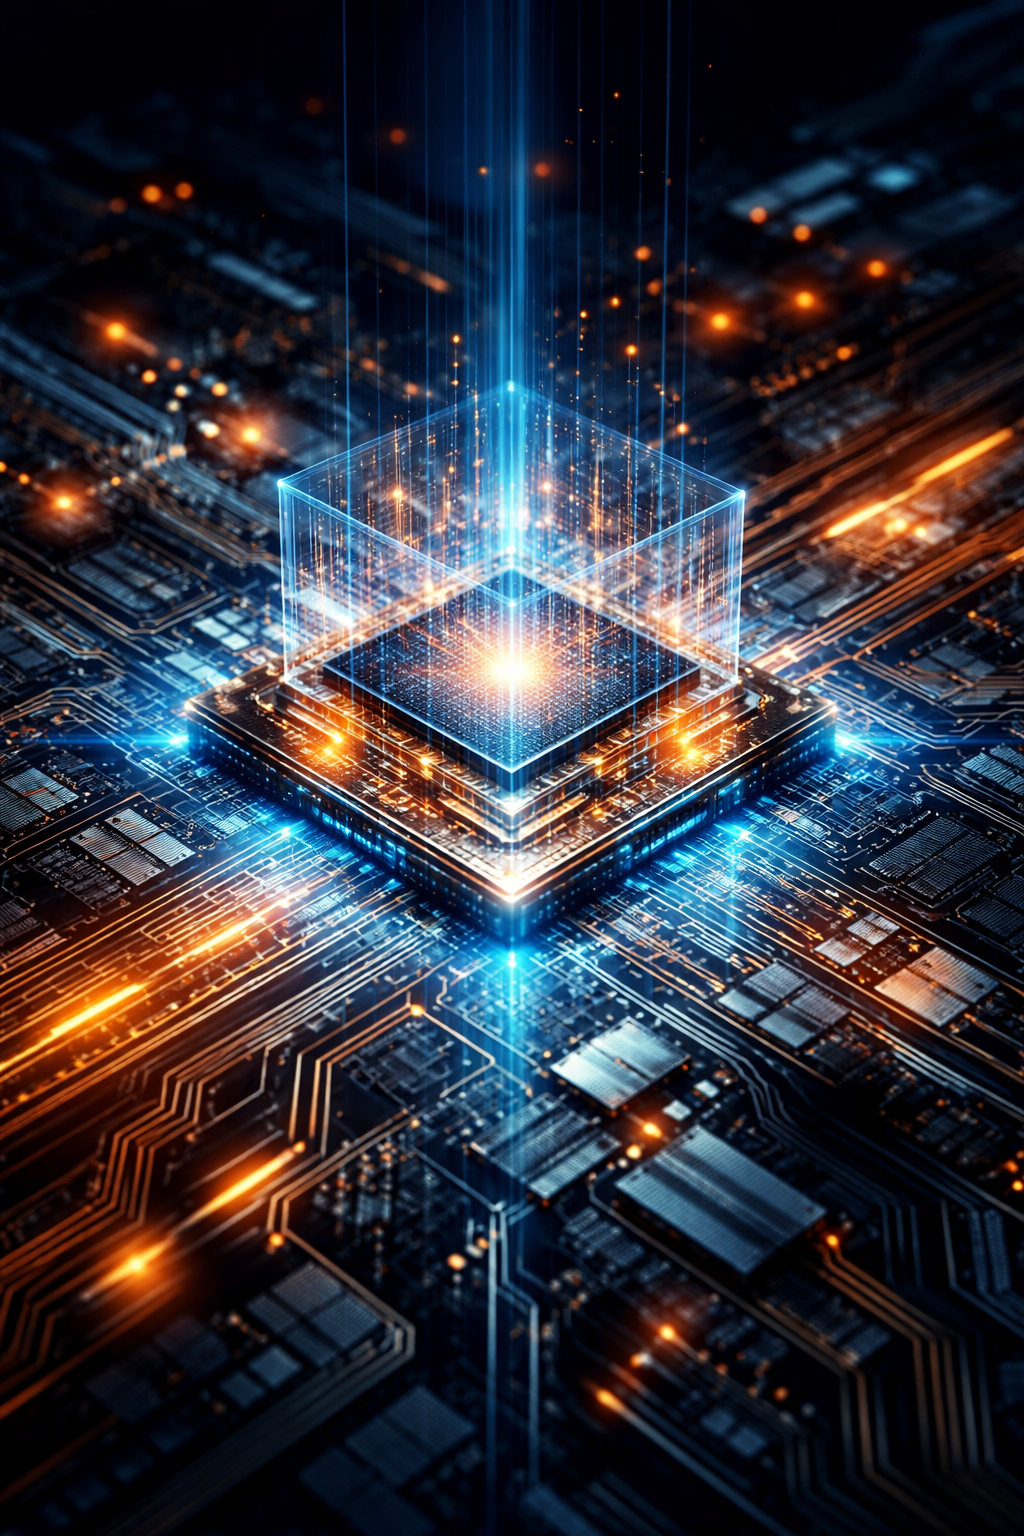
\includegraphics[width=\paperwidth]{gorseller/kapak-arkaplan.png}%
        };
    \end{scope}

    % === ALT BÖLGE: Koyu degrade (metin okunabilirliği için) ===
    % Alt %45: tamamen koyu
    \fill[pcbzemin, opacity=0.85]
        (current page.south west) rectangle ([yshift=13.5cm]current page.south east);
    % Kademeli geçiş bantları (yumuşak degrade etkisi)
    \fill[pcbzemin, opacity=0.7]
        ([yshift=13.5cm]current page.south west) rectangle ([yshift=14.5cm]current page.south east);
    \fill[pcbzemin, opacity=0.5]
        ([yshift=14.5cm]current page.south west) rectangle ([yshift=15.5cm]current page.south east);
    \fill[pcbzemin, opacity=0.3]
        ([yshift=15.5cm]current page.south west) rectangle ([yshift=16.5cm]current page.south east);
    \fill[pcbzemin, opacity=0.15]
        ([yshift=16.5cm]current page.south west) rectangle ([yshift=17.5cm]current page.south east);

    % === ÜST ŞERİT (ince altın çizgi) ===
    \fill[pcbaltin] (current page.north west) rectangle ([yshift=-1.2mm]current page.north east);

    % === ALT ŞERİT (ince altın çizgi) ===
    \fill[pcbaltin] ([yshift=1.2mm]current page.south west) rectangle (current page.south east);

    % === ANA BAŞLIK ===
    \node[font=\fontsize{42}{50}\selectfont\bfseries, text=pcbbeyaz]
        at ([yshift=9.5cm]current page.south) {Bilgisayar};
    \node[font=\fontsize{42}{50}\selectfont\bfseries, text=pcbbeyaz]
        at ([yshift=7.5cm]current page.south) {Mimarisi};

    % === ALTIN AYIRICI ÇİZGİ ===
    \draw[pcbaltin, line width=1.2pt]
        ([yshift=6.5cm, xshift=-3cm]current page.south) -- ++(6cm,0);

    % === ALT BAŞLIK ===
    \node[font=\Large\itshape, text=pcbacik]
        at ([yshift=5.5cm]current page.south) {RISC-V Tabanlı Yaklaşım};

    % === YAZAR ADI ===
    \node[font=\large\bfseries, text=pcbbeyaz]
        at ([yshift=3.8cm]current page.south) {Prof.\ Dr.\ Oğuz Ergin};

    % === BASKI BİLGİSİ ===
    \node[font=\normalsize, text=pcbaltin, opacity=0.7]
        at ([yshift=1.8cm]current page.south) {Sürüm 0.2.0\ \ $\cdot$\ \ \the\year};

\end{tikzpicture}
\vfill
\end{titlepage}


% ===== 2. KÜNYE =====
\cleardoublepage
\thispagestyle{empty}
\vspace*{\fill}
\noindent
{\small
\textbf{Bilgisayar Mimarisi} --- RISC-V Tabanlı Yaklaşım\\[3pt]
Prof.\ Dr.\ Oğuz Ergin\\[6pt]
Sürüm \kitapsurum, \the\year\\[12pt]
Bu kitap, lisans düzeyinde bilgisayar mimarisi derslerinde ders kitabı
olarak kullanılmak üzere hazırlanmıştır.\\[6pt]
Tüm hakları saklıdır.\\[24pt]
\textit{Bu dosya yayınevi değerlendirmesi için hazırlanmış tanıtım nüshasıdır.\\
Kitabın tamamı 12 bölüm, 4 ek ve yaklaşık 600 sayfadan oluşmaktadır.}
}
\vspace{2cm}

% ===== 3. ÖNSÖZ =====
\cleardoublepage
\chapter*{Önsöz}
\addcontentsline{toc}{chapter}{Önsöz}

Bu kitap, lisans düzeyindeki bilgisayar mimarisi derslerinde kaynak kitap olarak kullanılmak üzere hazırlanmıştır. Kitabın amacı, bilgisayar mühendisliği ve ilgili mühendislik dallarındaki öğrencilere, çağdaş bilgisayar sistemlerinin temel yapısını ve çalışma prensiplerini Türkçe olarak sunmaktır.

Kitap boyunca RISC-V buyruk kümesi mimarisi temel alınmıştır. RISC-V, açık kaynaklı ve modüler yapısıyla hem akademik hem de endüstriyel alanda giderek yaygınlaşan çağdaş bir mimaridir. Bu tercih, öğrencilerin güncel ve geleceğe yönelik bir mimari üzerinden kavramları öğrenmesini sağlamaktadır.

İlk bölümde bilgisayarların tarihsel gelişimi ve temel kavramlar ele alınmaktadır. İkinci bölümde başarım değerlendirmesi, üçüncü bölümde buyruk kümesi mimarisi, dördüncü bölümde RISC-V ile programlama, beşinci bölümde aritmetik işlemler, altıncı bölümde işlemci tasarımı ve yedinci bölümde boru hattı yöntemleri anlatılmaktadır. Sekizinci bölüm bellek hiyerarşisine, dokuzuncu bölüm giriş/çıkış sistemlerine ayrılmıştır. Onuncu bölümde çok çekirdekli işlemciler, on birinci bölümde GPU ve hızlandırıcılar, on ikinci bölümde ise güncel mimari eğilimleri tartışılmaktadır. Ek~A'da sayı sistemleri ve kodlama, Ek~B'de sayısal tasarım temelleri, Ek~C'de RISC-V referans kartı, Ek~D'de ise uygulamalı çalışma rehberi ve mini projeler sunulmaktadır.

Her bölümün başında, Türkiye'nin mimari mirasından bir eser fotoğrafı yer almaktadır. Bu eserler, bilgisayar mimarisi kavramlarıyla tematik bir bağ kurularak seçilmiştir.

Bu kitabın hazırlanmasında destek ve katkılarından dolayı Kasırga araştırma takımındaki öğrencilerime teşekkür ederim.

\vspace{1cm}
\begin{flushright}
\textit{Oğuz Ergin}\\
Ankara, \the\year
\end{flushright}
\cleardoublepage

% ===== 4. KİTABIN İÇERİĞİ (tam yapı özeti) =====
\chapter*{Kitabın İçeriği}
\addcontentsline{toc}{chapter}{Kitabın İçeriği}

\vspace{0.3cm}
\noindent
{\small\itshape Aşağıda kitabın tam içerik yapısı sunulmaktadır. Bu tanıtım dosyasında yalnızca Bölüm~1 örnek olarak yer almaktadır.}

\vspace{0.8cm}

\renewcommand{\arraystretch}{1.4}
\noindent
\begin{longtable}{@{}>{\bfseries\color{bolumrenk}}r@{\hspace{0.5cm}}p{12.8cm}}

\multicolumn{2}{@{}l}{\large\bfseries\color{bolumrenk} Ana Bölümler}\\[4pt]
\hline\\[-8pt]
\endfirsthead
\multicolumn{2}{@{}l}{\large\bfseries\color{bolumrenk} Kitabın İçeriği \textnormal{\textit{(devam)}}}\\[4pt]
\hline\\[-8pt]
\endhead

1 & \textbf{Bilgisayar Mimarisine Giriş}\\
  & {\small Bilgisayarların tarihsel gelişimi, Moore Yasası, işlemci ve yonga üretimi, programların çalıştırılması, güç tüketimi, RISC-V'e giriş, yapay zekâ ve mimari.}\\[2pt]

2 & \textbf{Bilgisayar Başarımı}\\
  & {\small Başarım ölçütleri, yürütme süresi, Amdahl Yasası, SPEC kıyaslama araçları, enerji verimliliği.}\\[2pt]

3 & \textbf{Buyruk Kümesi Mimarisi}\\
  & {\small RISC-V buyruk biçimleri, aritmetik ve mantık buyrukları, bellek erişimi, dallanma ve döngüler, yordamlar, yığın yapısı.}\\[2pt]

4 & \textbf{RISC-V ile Programlama}\\
  & {\small Çevirici dil programlama, yazmaç kullanım kuralları, yığın yönetimi, yordam çağrıları, dizgi ve dizi işlemleri, başarım çözümlemesi.}\\[2pt]

5 & \textbf{Aritmetik İşlemler}\\
  & {\small Toplama ve çıkarma devreleri, çarpma ve bölme algoritmaları, kayan nokta aritmetiği, IEEE~754 standardı.}\\[2pt]

6 & \textbf{İşlemci Tasarımı}\\
  & {\small Tek çevrimli ve çok çevrimli veri yolu tasarımı, denetim birimi, ALU tasarımı, durum makineleri.}\\[2pt]

7 & \textbf{Boru Hattı}\\
  & {\small Boru hattı kavramı, veri ve denetim sorunları, yönlendirme, dallanma öngörüsü, ileri boru hattı teknikleri.}\\[2pt]

8 & \textbf{Bellek}\\
  & {\small Bellek hiyerarşisi, önbellek tasarımı, sanal bellek, ESÖ (TLB), bellek tutarlılığı.}\\[2pt]

9 & \textbf{Giriş ve Çıkış Aygıtları}\\
  & {\small G/Ç arayüzleri, yol (bus) yapıları, kesmeler, DMA, disk ve depolama sistemleri.}\\[2pt]

10 & \textbf{Çok Çekirdekli ve Koşut İşlemciler}\\
  & {\small Koşut hesaplama, çok çekirdekli mimariler, önbellek tutarlılığı, MESI protokolü, bellek tutarlılık modelleri.}\\[2pt]

11 & \textbf{GPU ve Hızlandırıcılar}\\
  & {\small GPU mimarisi, SIMT modeli, CUDA programlama, alana özgü hızlandırıcılar, TPU.}\\[2pt]

12 & \textbf{Güncel Mimari Eğilimleri}\\
  & {\small RISC-V ekosistemi, ARM ve x86 karşılaştırması, yongacık yaklaşımı, kuantum hesaplama, güvenlik açıkları.}\\[6pt]

\multicolumn{2}{@{}l}{\large\bfseries\color{bolumrenk} Ekler}\\[4pt]
\hline\\[-8pt]

A & \textbf{Sayı Sistemleri ve Kodlama}\\
  & {\small İkili, sekizli, onaltılı sistemler; ikiye tümleyen, BCD, ASCII ve Unicode kodlama.}\\[2pt]

B & \textbf{Sayısal Tasarım Temelleri}\\
  & {\small Boole cebri, kapı devreleri, birleşik ve ardışıl mantık, sonlu durum makineleri.}\\[2pt]

C & \textbf{RISC-V Referans Kartı}\\
  & {\small RV32I buyruk tablosu, yazmaç haritası, buyruk biçimleri, sözde buyruklar.}\\[2pt]

D & \textbf{RISC-V Uygulama Çalışmaları ve Projeler}\\
  & {\small Ripes benzetimliği rehberi, örnek projeler, mini tasarım ödevleri.}\\[2pt]

\end{longtable}
\renewcommand{\arraystretch}{1.0}

\vspace{0.8cm}
\noindent
{\small\itshape Kitapta ayrıca Terimler Sözlüğü (İngilizce--Türkçe), Kaynakça, Önerilen Kaynaklar ve Dizin bölümleri bulunmaktadır. Her bölüm çok sayıda çözümlü örnek, şekil, tablo ve bölüm sonu alıştırması içermektedir.}

\cleardoublepage

% ===== 5. ÖRNEK BÖLÜM: Bölüm 1 =====
\mainmatter
% =============================================================
% Bölüm 1: Bilgisayar Mimarisine Giriş
% =============================================================
\chapter{Bilgisayar Mimarisine Giriş}
\label{chap:giris}
\bolumfoto{gorseller/bolum01-ayasofya.jpg}{Ayasofya -- İstanbul}

\section{Giriş}
\label{sec:giris}

Cebinizdeki akıllı telefon, 1969'da insanı Ay'a götüren Apollo rehberlik bilgisayarından milyonlarca kat daha güçlü. Bugün bilgisayarlar yalnızca masaüstünde değil, saatimizde, buzdolabımızda, otomobilimizde ve veri merkezlerindeki devasa sunucu çiftliklerinde karşımıza çıkıyor. Bu yaygınlığın arkasında yarım yüzyılı aşan sürekli bir mimari yenilenme var.

\emph{Bilgisayar mimarisi}\index{bilgisayar mimarisi}, donanım ile yazılım arasındaki sınırı tanımlayan ve işlemci, bellek ve giriş/çıkış birimlerinin nasıl bir araya geleceğini belirleyen mühendislik dalıdır. Verimli yazılım geliştirmek isteyen bir programcı için donanımın çalışma ilkelerini anlamak, yüksek başarımlı donanım tasarlamak isteyen bir mühendis için de yazılım gereksinimlerini kavramak vazgeçilmez. Üstelik alan, tarihsel bir dönüm noktasında: transistörler küçüldükçe güç yoğunluğunun sabit kalacağını öngören Dennard ölçeklemesinin\index{Dennard ölçeklemesi} sona ermesi, yapay zekânın yükselişi ve açık kaynak donanım hareketleri bilgisayar mimarisini her zamankinden daha heyecanlı bir araştırma alanı yapıyor.

Bu bölümde önce bilgisayarların tarihsel gelişimini, ardından bir bilgisayarın temel bileşenlerini ve işlemcinin nasıl üretildiğini göreceğiz. Sonra programların bu donanım üzerinde nasıl çalıştırıldığını, mimariyi şekillendiren etkenleri, güç tüketimi sorununu, RISC-V buyruk kümesinin neden tercih edildiğini ve yapay zekânın bilgisayar mimarisine getirdiği yeni ufukları ele alacağız.



\section{Bilgisayarların Gelişimi}
\label{sec:bilgisayar-gelisimi}

Abaküsle başlayan hesap yapma gereksinimi, önce mekanik, sonra da elektronik hesap makineleriyle karşılanmaya çalışıldı. Bilinen anlamda ilk mekanik hesap makinesini Blaise Pascal\index{Pascal, Blaise} 1642'de tasarladı. Pascal, toplama ve çıkarma işlemlerini yapabilen bu makineyi vergi tahsildarı babasına yardım etmek amacıyla geliştirdi. Şekil~\ref{fig:pascal-makine}'de Pascal'ın yaptığı bu ilk makinenin bir resmi görülüyor.

\begin{figure}[H]
\centering
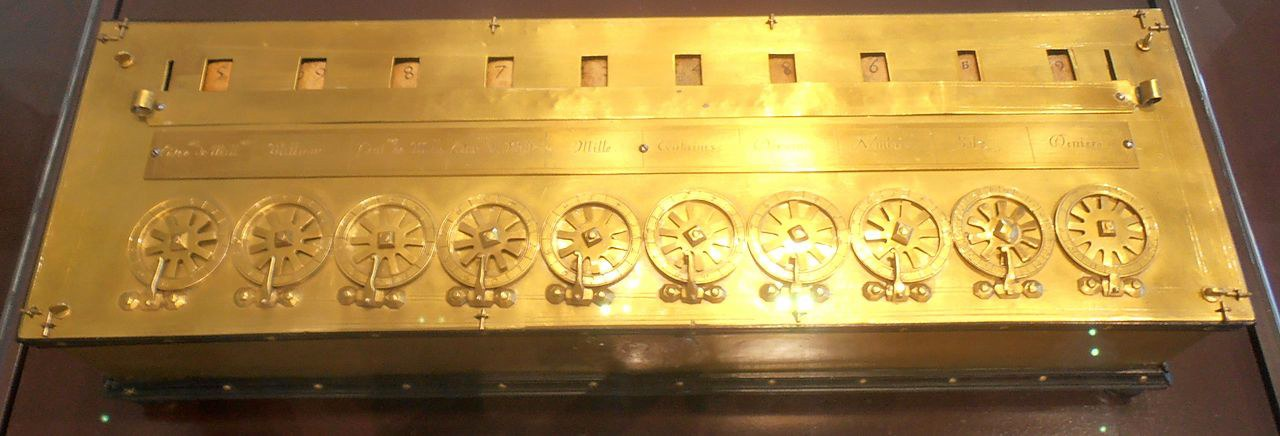
\includegraphics[width=0.85\textwidth]{gorseller/pascaline.jpg}
\caption{Blaise Pascal'ın 1642'de yaptığı mekanik hesap makinesi (Pascaline)}
\label{fig:pascal-makine}
\end{figure}

19.~yüzyılın sonlarından itibaren hesaplama makineleri hızla gelişti. 1890'da Herman Hollerith\index{Hollerith, Herman} delikli kart sistemiyle çalışan bir hesaplama düzeneği geliştirdi; bu sistem ABD nüfus sayımında başarıyla kullanıldı.

Bu gelişmelere paralel olarak Alan Turing\index{Turing, Alan} 1936'da yayımladığı makalesinde~\cite{turing1936}, sonradan \emph{Turing makinesi}\index{Turing makinesi} olarak anılacak soyut hesaplama modelini tanımlayarak hesaplanabilirliğin\index{hesaplanabilirlik} teorik temelini attı. Bu model, bir algoritma ile çözülebilecek her problemin basit bir bant, okuma/yazma kafası ve sonlu durum tablosundan oluşan bir makineyle çözülebileceğini gösteriyordu. Turing makinesi kavramı, bilgisayar biliminin kurucu taşlarından biri olarak kabul edilir ve günümüzde bile algoritma karmaşıklığı ve hesaplanabilirlik kuramının temelini oluşturur.

2.~Dünya Savaşı döneminde hesaplama ihtiyacı iyice arttı ve birçok öncü makine üretildi. Turing, İngiltere'de Bletchley Park'ta\index{Bletchley Park} Alman Enigma\index{Enigma} şifre makinesinin kırılması için elektro-mekanik Bombe\index{Bombe} makinesini tasarladı. İngilizler daha sonra daha gelişmiş şifrelerin çözümü için Colossus\index{Colossus}'u geliştirdi. Aynı dönemde IBM ile çalışan Howard H.~Aiken\index{Aiken, Howard H.} 1944'te rölelerden oluşan Mark~I\index{Mark I}'i tasarladı. Bilgisayar tarihinin sonraki dönüm noktaları aşağıda nesiller halinde ele alınıyor.

\subsubsection*{Birinci Nesil: Vakum Tüpleri (1940'lar--1950'ler)}
Günümüz bilgisayarlarının atası sayılan ENIAC\index{ENIAC} (Electronic Numerical Integrator And Computer), 1945'te Pennsylvania Üniversitesi'nde tamamlandı. 19.000 vakum tüpü\index{vakum tüpü} kullanan, 30~tonluk ve 200~kW güç tüketen bu dev makine yalnızca dört işlem ve basit karşılaştırma yapabiliyordu. Kısa süre sonra Von Neumann'ın\index{Von Neumann} teorik katkılarıyla tasarlanan EDVAC\index{EDVAC}, programı ve veriyi aynı bellekte saklayarak çığır açtı. Birinci nesil bilgisayarlar makine dili\index{makine dili} ile programlanıyordu; vakum tüplerinin kısa ömrü, büyük boyutu ve yüksek ısı üretimi en önemli sınırlılıkları oluşturuyordu.

\subsubsection*{İkinci Nesil: Transistörler (1950'ler--1960'lar)}
1947'de Bell Laboratuvarları'nda William Shockley, John Bardeen ve Walter Brattain tarafından icat edilen transistör\index{transistör}, vakum tüplerinin yerini aldı. Transistörler çok daha küçük, güvenilir ve ucuzdu; güç tüketimleri de düşüktü. Bu dönemde çevirici dil\index{çevirici dil} (Assembly\index{Assembly}) kullanılmaya başlandı ve programlama önemli ölçüde kolaylaştı. Fortran ve COBOL gibi ilk üst düzey diller de bu nesilde ortaya çıktı.

\subsubsection*{Üçüncü Nesil: Tümleşik Devreler (1960'lar--1970'ler)}
Texas Instruments'ta Jack Kilby\index{Kilby, Jack} ve Intel'de Robert Noyce\index{Noyce, Robert} birbirinden bağımsız olarak tümleşik devreyi\index{tümleşik devre} geliştirdi. Tüm bileşenlerin ve bağlantıların aynı yarıiletken malzeme üzerinde üretilmesi, devrelerin boyutunu ve maliyetini büyük ölçüde düşürdü. Bu dönemde işletim sistemleri\index{işletim sistemi} yaygınlaştı ve birden çok programın aynı belleği paylaşması mümkün hale geldi.

\subsubsection*{Dördüncü Nesil: Mikroişlemciler (1970'ler--2000'ler)}
1971'de Intel'in 4004\index{Intel 4004} yongası, işlemcinin tüm bileşenlerini tek bir tümleşik devre üzerinde toplayan ilk \emph{mikroişlemci}\index{mikroişlemci} oldu. Moore yasasının\index{Moore yasası} öngördüğü transistör artışı sayesinde işlemciler hızla güçlendi; 1981'de kişisel bilgisayar\index{kişisel bilgisayar} (PC) kavramı doğdu ve bilgisayarlar geniş kitlelere ulaştı. Bu nesil boyunca saat sıklığı sürekli artırılarak başarım kazanımı sağlandı.

\subsubsection*{Beşinci Nesil: Çok Çekirdekli ve Heterojen Mimariler (2000'ler--günümüz)}
2000'li yılların ortalarından itibaren güç duvarı\index{güç duvarı} ve Dennard ölçeklemesinin\index{Dennard ölçeklemesi} sona ermesi saat sıklığını artırma stratejisini sürdürülemez kıldı. Tasarımcılar, tek bir yonga üzerine birden çok çekirdek\index{çok çekirdekli} yerleştirerek başarım artışını paralel hesaplamaya kaydırdı. Günümüzde CPU çekirdeklerinin yanına GPU\index{GPU}, NPU\index{NPU} ve diğer özelleşmiş hızlandırıcılar eklenerek \emph{heterojen} mimariler oluşturuluyor. Açık kaynaklı RISC-V\index{RISC-V} buyruk kümesi mimarisi de bu dönemin önemli gelişmeleri arasında yer alıyor.

\begin{bilginot}[Robert Dennard ve Dennard Ölçeklemesi]
IBM araştırmacısı Robert Dennard\index{Dennard, Robert}, 1974'te yayımladığı makalede~\cite{dennard1974} transistör boyutlarının küçültülmesinin etkilerini inceledi. Dennard'ın ortaya koyduğu ölçekleme kuralına göre transistörler küçüldükçe çalışma gerilimleri ve akımları da orantılı biçimde azalır; dolayısıyla birim alan başına güç tüketimi yaklaşık sabit kalır. Bu ilke sayesinde 1970'lerden 2000'lerin başına kadar her yeni üretim teknolojisiyle hem daha fazla transistör sığdırılabildi hem de saat sıklığı artırılabildi --- çünkü ek transistörler fazladan güç tüketmiyordu. Ancak 2006 civarında transistör boyutları 65~nm'nin altına indiğinde sızıntı akımları\index{sızıntı akımı} baskın hale geldi ve Dennard ölçeklemesi geçerliliğini yitirdi. Bu dönüm noktası, işlemci tasarımında saat sıklığı yarışının sona ermesine ve çok çekirdekli mimarilere geçişe yol açtı.
\end{bilginot}

\begin{terimnotu}
\textbf{donanım} (\emph{hardware})\,: \emph{Donanmak} (to equip) fiilinden \emph{-ım} ekiyle. Bilgisayarın fiziksel ``donanımı'', tıpkı bir geminin donanması gibi.

\textbf{yazılım} (\emph{software})\,: \emph{Yazılmak} (to be written) fiilinin edilgen biçiminden \emph{-ım} ekiyle. Donanımın üzerinde çalışan ``yazılmış'' programlar.

\textbf{yonga} (\emph{chip})\,: \emph{Yontmak} (to carve, to whittle) fiilinin kökü \emph{yon-} ve \emph{-ga} ekiyle; ağaçtan yontularak çıkarılan ince parça demektir. İngilizce \emph{chip} de ``koparılan küçük parça'' anlamındadır. Paketlenmiş tümleşik devreyi ifade eder.

\textbf{kırmık} (\emph{die})\,: \emph{Kırmak} (to break) fiilinden \emph{-ık} ekiyle; silisyum dilimden (wafer) kesilerek ``kırılıp'' ayrılan, henüz paketlenmemiş yarı iletken parçasıdır.

\textbf{bellek} (\emph{memory})\,: \emph{Bellemek} (to memorize) fiilinden \emph{-ek} araç yapım ekiyle; ``belleme aracı'' demektir. Yazar Nurullah Ataç'ın önerisiyle Türkçeye kazandırılmış, Arapça kökenli \emph{hafıza} sözcüğünün yerini almıştır.

\textbf{tümleşik devre} (\emph{integrated circuit})\,: \emph{Tümleşmek} (to integrate, to merge into a whole) fiilinden; tüm bileşenlerin tek bir ``bütün'' haline getirildiği devre.
\end{terimnotu}

\subsection{Moore Yasası ve Transistör Artışı}
\label{sec:moore-yasasi}

Bu beş nesil boyunca yaşanan hızlı gelişimin arkasında, transistör teknolojisindeki üstel ilerleme yatıyor. Intel marka işlemcilerin tarihte gelişimi Tablo~\ref{tab:intel-gelisim}'de veriliyor.

\begin{table}[ht!]
\centering
\caption{Intel işlemcilerin gelişimi}
\label{tab:intel-gelisim}
\footnotesize
\begin{tabular}{llllp{5cm}}
\toprule
\textbf{Yonga} & \textbf{Tarih} & \textbf{Saat Sıklığı} & \textbf{Transistör Sayısı} & \textbf{Açıklama} \\
\midrule
4004       & 1971 & 0,108 MHz  & 2.300   & Bir yongadaki ilk mikroişlemci \\
8008       & 1972 & 0,108 MHz  & 3.500   & İlk 8 bitlik mikroişlemci \\
8080       & 1974 & 2 MHz      & 6.000   & İlk genel amaçlı işlemci \\
8086       & 1978 & 5--10 MHz  & 29.000  & İlk 16 bitlik mikroişlemci \\
8088       & 1979 & 5--8 MHz   & 29.000  & IBM PC'de kullanılan işlemci \\
80286      & 1982 & 8--12 MHz  & 134.000 & Bellek koruması bulunur \\
80386      & 1985 & 16--33 MHz & 275.000 & İlk 32 bitlik mikroişlemci \\
80486      & 1989 & 25--100 MHz& 1,2M    & 8 KB önbelleğe sahip \\
Pentium    & 1993 & 60--233 MHz& 3,1M    & İki boru hattı; MMX \\
Pentium Pro& 1995 & 150--200 MHz& 5,5M   & İki düzey önbellek \\
Pentium II & 1997 & 233--400 MHz& 7,5M   & Pentium Pro + MMX \\
Pentium III& 1999 & 500 MHz    & 9,5M    & Güç tasarrufu seviyeleri \\
Pentium 4  & 2000 & 1,5 GHz    & 42M     & Nanoteknoloji ile üretim \\
Pentium D  & 2005 & 3,2 GHz    & 291M    & İlk 2 çekirdekli masaüstü \\
Core 2 Duo & 2006 & 2,93 GHz   & 291M    & Pentium M'in gelişmiş hali \\
Quad Core  & 2007 & $>$3 GHz   & 410M    & İki tane Core 2 Duo \\
Xeon       & 2009 & 2,26 GHz   & 781M    & Ölçeklenebilirlik odaklı \\
Sandy Bridge & 2011 & 3,4 GHz   & 1,16Mr & AVX, tümleşik GPU \\
Haswell    & 2013 & 3,5 GHz    & 1,4Mr  & AVX2, FMA3 \\
Skylake    & 2015 & 4,0 GHz    & 1,75Mr & DDR4 desteği \\
Coffee Lake& 2018 & 3,6 GHz    & ${\sim}$3Mr & İlk 6 çekirdekli masaüstü \\
Alder Lake & 2021 & 5,2 GHz    & ${\sim}$10Mr & İlk karma mimari (P+E çekirdek) \\
Raptor Lake& 2022 & 5,8 GHz    & ${\sim}$26Mr & 8P+16E çekirdek \\
\bottomrule
\multicolumn{5}{l}{\scriptsize M = milyon; Mr = milyar; ``${\sim}$'' tahminî değer.}
\end{tabular}
\end{table}

Intel'in kurucularından Gordon Moore\index{Moore, Gordon} 1965 yılında bir kural ortaya attı: Her 1,5 yılda bir yonga başına kullanılan transistör sayısı 2 katına çıkacak. ``Moore Yasası''\index{Moore yasası} olarak bilinen bu kural fizik yasaları gibi değişmez bir gerçek değil. Ancak firmalar bu yasayı tasarımda kolaylık sağlayan ve geliştirme hedefi belirleyen bir kural olarak kabul ediyor. Tablodaki veriler incelendiğinde, 1971'den 2022'ye kadar transistör sayısının yaklaşık 10 milyon kat arttığı görülür. Bu büyüme hızı, insan uygarlığının başka hiçbir teknoloji alanında gözlemlenmemiştir. Şekil~\ref{fig:moore-yasasi}'de bu büyümenin logaritmik ölçekteki grafiği verilmiştir.

\begin{figure}[ht!]
\centering
\begin{tikzpicture}[>=Stealth, x=0.22cm, y=1.15cm]
    % Eksen aralıkları: X -> 1970-2025, Y -> log10 ölçeği (10^3 ile 10^11 arası)
    % Y konumu: log10(transistör) - 3  =>  10^3->0, 10^4->1, ..., 10^11->8

    % Y ekseni
    \draw[thick, ->] (1968,0) -- (1968,8.8) node[above, font=\small\bfseries] {Transistör Sayısı};
    % Y ekseni etiketleri
    \foreach \lev/\lab in {0/$10^3$, 1/$10^4$, 2/$10^5$, 3/$10^6$, 4/$10^7$, 5/$10^8$, 6/$10^9$, 7/$10^{10}$, 8/$10^{11}$} {
        \draw (1968,\lev) -- +(-0.8,0);
        \node[left, font=\footnotesize] at (1967.2,\lev) {\lab};
    }
    % Y ekseni ızgara çizgileri
    \foreach \lev in {0,1,...,8} {
        \draw[gray!25, thin] (1968,\lev) -- (2026,\lev);
    }

    % X ekseni
    \draw[thick, ->] (1968,0) -- (2027,0) node[right, font=\small\bfseries] {Yıl};
    % X ekseni etiketleri
    \foreach \yr in {1970,1975,...,2025} {
        \draw (\yr,0) -- ++(0,-0.15);
        \node[below, font=\footnotesize] at (\yr,-0.15) {\yr};
    }

    % Veri noktaları: (yıl, log10(transistör)-3)
    % 4004: 1971, 2300 -> log10(2300)=3.362 -> y=0.362
    % 8080: 1974, 6000 -> log10(6000)=3.778 -> y=0.778
    % 8086: 1978, 29000 -> log10(29000)=4.462 -> y=1.462
    % 80286: 1982, 134000 -> log10(134000)=5.127 -> y=2.127
    % 80386: 1985, 275000 -> log10(275000)=5.439 -> y=2.439
    % 80486: 1989, 1200000 -> log10(1.2M)=6.079 -> y=3.079
    % Pentium: 1993, 3100000 -> log10(3.1M)=6.491 -> y=3.491
    % Pentium III: 1999, 9500000 -> log10(9.5M)=6.978 -> y=3.978
    % Pentium 4: 2000, 42000000 -> log10(42M)=7.623 -> y=4.623
    % Core 2 Duo: 2006, 291000000 -> log10(291M)=8.464 -> y=5.464
    % Quad Core: 2007, 410000000 -> log10(410M)=8.613 -> y=5.613
    % Sandy Bridge: 2011, 1.16e9 -> log10=9.064 -> y=6.064
    % Haswell: 2013, 1.4e9 -> log10=9.146 -> y=6.146
    % Coffee Lake: 2018, 3e9 -> log10=9.477 -> y=6.477
    % Alder Lake: 2021, 1e10 -> log10=10.0 -> y=7.0
    % Raptor Lake: 2022, 2.6e10 -> log10=10.415 -> y=7.415

    % Eğilim çizgisi (yaklaşık Moore Yasası: her 1.5 yılda 2x)
    % 1971'de y=0.362, eğim = log10(2)/1.5 = 0.2007/yıl
    % 2024'te: 0.362 + (2024-1971)*0.2007 = 0.362 + 10.637 = 10.999
    \draw[dashed, sinyalkirmizi, thick] (1971, 0.362) -- (2024, 8.5)
        node[above left, font=\footnotesize, text=sinyalkirmizi] {Moore Yasası};

    % Noktalar ve etiketler
    \filldraw[sinyalmavi] (1971, 0.362) circle (2.5pt)
        node[above right, font=\scriptsize] {4004};
    \filldraw[sinyalmavi] (1974, 0.778) circle (2.5pt)
        node[above right, font=\scriptsize] {8080};
    \filldraw[sinyalmavi] (1978, 1.462) circle (2.5pt)
        node[above right, font=\scriptsize] {8086};
    \filldraw[sinyalmavi] (1982, 2.127) circle (2.5pt)
        node[above right, font=\scriptsize] {80286};
    \filldraw[sinyalmavi] (1985, 2.439) circle (2.5pt)
        node[above left, font=\scriptsize] {80386};
    \filldraw[sinyalmavi] (1989, 3.079) circle (2.5pt)
        node[above right, font=\scriptsize] {80486};
    \filldraw[sinyalmavi] (1993, 3.491) circle (2.5pt)
        node[above right, font=\scriptsize] {Pentium};
    \filldraw[sinyalmavi] (1999, 3.978) circle (2.5pt)
        node[above left, font=\scriptsize] {Pentium III};
    \filldraw[sinyalmavi] (2000, 4.623) circle (2.5pt)
        node[right, font=\scriptsize] {Pentium 4};
    \filldraw[sinyalmavi] (2006, 5.464) circle (2.5pt)
        node[above left, font=\scriptsize] {Core 2 Duo};
    \filldraw[sinyalmavi] (2007, 5.613) circle (2.5pt)
        node[below right, font=\scriptsize] {Quad Core};
    \filldraw[sinyalmavi] (2011, 6.064) circle (2.5pt)
        node[above left, font=\scriptsize] {Sandy Bridge};
    \filldraw[sinyalmavi] (2013, 6.146) circle (2.5pt)
        node[below right, font=\scriptsize] {Haswell};
    \filldraw[sinyalmavi] (2018, 6.477) circle (2.5pt)
        node[below right, font=\scriptsize] {Coffee Lake};
    \filldraw[sinyalmavi] (2021, 7.0) circle (2.5pt)
        node[above left, font=\scriptsize] {Alder Lake};
    \filldraw[sinyalmavi] (2022, 7.415) circle (2.5pt)
        node[right, font=\scriptsize] {Raptor Lake};

    % Noktaları birleştiren çizgi
    \draw[sinyalmavi, thin]
        (1971, 0.362) -- (1974, 0.778) -- (1978, 1.462) --
        (1982, 2.127) -- (1985, 2.439) -- (1989, 3.079) --
        (1993, 3.491) -- (1999, 3.978) -- (2000, 4.623) --
        (2006, 5.464) -- (2007, 5.613) -- (2011, 6.064) --
        (2013, 6.146) -- (2018, 6.477) -- (2021, 7.0) --
        (2022, 7.415);
\end{tikzpicture}
\caption[Intel işlemcilerdeki transistör sayısının artışı]{Yıllara göre Intel işlemcilerdeki transistör sayısının artışı (grafik logaritmik ölçektedir). Kesik çizgi Moore Yasası'nın öngördüğü eğilimi göstermektedir.}
\label{fig:moore-yasasi}
\end{figure}

\begin{bilginot}[Moore Yasası'nın Geleceği]
Moore Yasası, yarım yüzyılı aşkın bir süre endüstrinin yol haritasını belirledi. Ancak transistör boyutları atom ölçeğine yaklaştıkça (3~nm ve altı) fiziksel sınırlar belirginleşiyor. Dennard ölçeklemesinin de sona ermesiyle birlikte saat sıklığını artırma stratejisi sürdürülemez hale geldi ve tasarımcılar çok çekirdekli ve heterojen mimarilere yöneldi. Günümüzde başarım artışı, tek çekirdeğin hızlandırılması yerine paralel hesaplama ve özel amaçlı hızlandırıcılarla (GPU, TPU, NPU) sağlanıyor.
\end{bilginot}

\section{Bilgisayar Nedir?}
\label{sec:bilgisayar-nedir}

Bilgisayar veri alabilen, aldığı veriler üzerinde işlemler yapan ve sonuç üreten bir makinedir. Bilgisayarlar veri yolu, denetim, bellek, giriş ve çıkış olmak üzere beş ana bileşenden oluşur. Şekil~\ref{fig:bes-bilesen}'te gösterildiği üzere veri yolu ve denetim birimleri işlemciyi oluşturur.

\begin{figure}[H]
\centering
\begin{tikzpicture}[>=Stealth, scale=0.88, every node/.style={scale=0.88},
    bilesen/.style={draw, thick, rounded corners=3pt, minimum height=1.1cm, align=center, font=\small}]

    % === İşlemci çerçevesi ===
    \node[draw, very thick, rounded corners=5pt, minimum width=7.6cm, minimum height=2.0cm,
          fill=blokmavi-acik, dashed] (islemci) {};
    \node[font=\small\bfseries, anchor=north] at ([yshift=2pt]islemci.north) {İşlemci (\emph{Processor})};

    % Veri Yolu (sol iç blok)
    \node[bilesen, fill=blokmavi, minimum width=2.8cm]
          at ([xshift=-1.4cm, yshift=-0.1cm]islemci.center) (veriyolu) {\textbf{Veri Yolu}\\[-2pt]{\scriptsize\itshape Datapath}};
    % Denetim (sağ iç blok)
    \node[bilesen, fill=blokkirmizi-acik, minimum width=2.8cm]
          at ([xshift=1.4cm, yshift=-0.1cm]islemci.center) (denetim) {\textbf{Denetim}\\[-2pt]{\scriptsize\itshape Control}};
    % Veri yolu <-> Denetim iç bağlantısı (ince çizgi, açıklayıcı)
    \draw[-, thin, gray!60] (veriyolu.east) -- (denetim.west);

    % === Bellek (üstte) ===
    \node[bilesen, fill=bloksari, minimum width=3.2cm,
          above=0.7cm of islemci]
          (bellek) {\textbf{Bellek}\\[-2pt]{\scriptsize\itshape Memory}};

    % === Giriş (sol altta) ===
    \node[bilesen, fill=blokyesil-acik, minimum width=2.4cm,
          below left=0.7cm and 0.1cm of islemci]
          (giris) {\textbf{Giriş}\\[-2pt]{\scriptsize\itshape Input}};

    % === Çıkış (sağ altta) ===
    \node[bilesen, fill=blokyesil-acik, minimum width=2.4cm,
          below right=0.7cm and 0.1cm of islemci]
          (cikis) {\textbf{Çıkış}\\[-2pt]{\scriptsize\itshape Output}};

    % === Bağlantı çizgileri ===
    % İşlemci <-> Bellek
    \draw[<->, very thick, sinyalmavi] (islemci.north) -- (bellek.south);

    % Giriş -> İşlemci
    \draw[->, very thick, sinyalmavi] (giris.north) -- ([xshift=-1.2cm]islemci.south);

    % İşlemci -> Çıkış
    \draw[->, very thick, sinyalmavi] ([xshift=1.2cm]islemci.south) -- (cikis.north);

    % Giriş -> Bellek (sol taraftan)
    \draw[->, thick, gray] (giris.west) -- ++(-0.5,0) |- (bellek.west);

    % Bellek -> Çıkış (sağ taraftan)
    \draw[->, thick, gray] (bellek.east) -| ([xshift=0.5cm]cikis.east) -- (cikis.east);

\end{tikzpicture}
\vspace{-2mm}
\caption{Bilgisayarın 5 ana bileşeni}
\label{fig:bes-bilesen}
\end{figure}

\subsection{Bilgisayarın Parçaları}
\label{sec:bilgisayar-parcalari}

Günümüzde ``bilgisayar'' kavramı yalnızca masaüstü ya da dizüstü bilgisayarlarla sınırlı değil. Akıllı telefonlar, tabletler, akıllı saatler, sunucular ve araç içi gömülü sistemler de birer bilgisayar. Boyutları ve kullanım alanları farklı olsa da tüm bu aygıtlar Şekil~\ref{fig:bes-bilesen}'te gösterilen beş temel bileşeni içerir.

\subsubsection*{İşlemci}
Bilgisayarın beyni olan \emph{işlemci}\index{işlemci} (\emph{processor}), programdaki buyrukları yürüten birimdir. Şekil~\ref{fig:bes-bilesen}'te görüldüğü gibi işlemci iki alt birimden oluşur: \textbf{veri yolu}\index{veri yolu} (\emph{datapath}) ve \textbf{denetim}\index{denetim birimi} (\emph{control}). Veri yolu, aritmetik ve mantık işlemlerini gerçekleştiren donanım yollarını --- toplayıcılar, yazmaçlar, çoklayıcılar gibi birimleri --- barındırır. Denetim birimi ise her buyruğun hangi adımda ne yapacağını belirleyen sinyalleri üretir; bir orkestra şefi gibi veri yolundaki birimlerin doğru zamanda doğru işi yapmasını sağlar. İşlemci tasarımı Bölüm~\ref{chap:islemci-tasarimi}'te, boru hattıyla başarım artırma teknikleri ise Bölüm~\ref{chap:boruhatti}'da ayrıntılı olarak ele alınacaktır.

\subsubsection*{Bellek}
Programların ve verilerin saklandığı bileşene \emph{bellek}\index{bellek} denir. Bilgisayarlarda iki temel bellek türü bulunur: uçucu (\emph{volatile}) ve uçucu olmayan (\emph{non-volatile}). Uçucu bellekler --- örneğin DRAM --- güç kesildiğinde içeriklerini kaybeder ve program çalışırken veriye hızlı erişim sağlamak için kullanılır. Uçucu olmayan bellekler ise --- SSD, sabit disk gibi --- güç olmadan da veriyi korur ve kalıcı depolama için tercih edilir. Bellek hiyerarşisi, hız ve maliyet dengesini sağlamak amacıyla farklı türdeki belleklerin katmanlı biçimde düzenlenmesiyle oluşturulur; bu konu Bölüm~\ref{chap:bellek}'de ayrıntılı olarak ele alınacaktır.

\subsubsection*{Giriş aygıtları}
Bilgisayara veri sağlayan birimlere \emph{giriş aygıtı}\index{giriş aygıtı} denir. Klavye ve fare onlarca yıldır en yaygın giriş aygıtları olmuştur; akıllı telefonlarda ise dokunmatik ekran hem giriş hem çıkış işlevi görür. Bunların yanı sıra ivme ölçer, GPS alıcısı ve parmak izi okuyucu gibi çeşitli algılayıcılar da birer giriş aygıtıdır.

Yapay zekâ çağıyla birlikte \emph{mikrofon}\index{mikrofon} ve \emph{kamera}\index{kamera} giderek daha önemli giriş aygıtları hâline geliyor. Büyük dil modelleri ve konuşma tanıma sistemleri sayesinde kullanıcılar bilgisayarla doğal dilde sesli iletişim kurabiliyor. Kameralar ise yalnızca fotoğraf çekmekle kalmayıp, yapay zekâ destekli görüntü anlama, yüz tanıma, hareket algılama ve artırılmış gerçeklik gibi uygulamalara girdi sağlıyor. Bu eğilim, mikrofon ve kameranın yakın gelecekte klavye ve farenin önüne geçeceğine işaret ediyor.

Giriş aygıtlarının hızları birbirinden çok farklıdır. Bir klavye saniyede birkaç bayt üretirken, bir mikrofon saniyede on binlerce ses örneği (\emph{sample}) üretir --- örneğin 16 bit, 48\,kHz örnekleme ile saniyede yaklaşık 96\,KB. Yüksek çözünürlüklü bir kamera ise saniyede gigabaytlar düzeyinde ham veri üretebilir. Bu büyük hız farkı, giriş/çıkış alt sisteminin tasarımında kritik bir etkendir ve Bölüm~\ref{chap:giris-cikis}'de ayrıntılı olarak ele alınacaktır.

\subsubsection*{Çıkış aygıtları}
İşlenen verilerin kullanıcıya ya da başka bir sisteme iletilmesini sağlayan birimlere \emph{çıkış aygıtı}\index{çıkış aygıtı} denir. Monitör (LCD, OLED) ve yazıcı en bilinen görsel çıkış aygıtlarıdır. Bir beneğin (\emph{pixel}) rengini göstermek için kırmızı, yeşil ve mavi kanalların her birine 8 bit ayrılır; dolayısıyla bir beneğin rengi 24 bitle ifade edilir. 1920$\times$1080 çözünürlükteki bir ekranda yaklaşık 2 milyon benek bulunur ve bunların tamamının saniyede en az 60 kez yenilenmesi gerekir; bu da grafik alt sisteminden yüksek bir veri aktarım hızı talep eder.

Yapay zekânın yaygınlaşmasıyla birlikte \emph{hoparlör}\index{hoparlör} de en az ekran kadar önemli bir çıkış aygıtı hâline gelmiştir. Yapay zekâ destekli konuşma sentezi (\emph{text-to-speech}) teknolojileri artık insandan ayırt edilemeyecek kadar doğal ses üretebiliyor. Akıllı hoparlörler, araç içi asistanlar ve giyilebilir aygıtlar gibi ekranı küçük ya da hiç olmayan sistemlerde ses, birincil çıkış kanalı olarak öne çıkıyor. Böylece giriş tarafında mikrofon ve kamera, çıkış tarafında ise hoparlör ve ekran birlikte çalışarak insanla bilgisayar arasında çok kipli (\emph{multimodal})\index{çok kipli etkileşim} bir etkileşim ortamı oluşturuyor.

\subsubsection*{Ana kart}
Bilgisayarın bileşenlerini birbirine bağlayan ve uyumlu çalışmalarını sağlayan donanıma \emph{ana kart}\index{ana kart} denir. Ana kart üzerinde işlemci yuvası, bellek yuvaları, giriş/çıkış denetleyicileri, genişleme yuvaları ve çeşitli bağlantı arabirimleri bulunur. Bileşenler arasındaki veri akışı, ana kart üzerindeki \emph{yol}\index{yol} (\emph{bus}) adı verilen iletişim hatları aracılığıyla sağlanır. Modern ana kartlarda yüksek hızlı bileşenler için ayrı bir kuzey köprüsü, düşük hızlı bileşenler için ise güney köprüsü kullanılırdı; günümüzde bu işlevlerin çoğu doğrudan işlemci içine entegre edilmiştir.

\subsubsection*{Bilgisayar türleri}
Yukarıda tanımlanan beş temel bileşen --- işlemci, bellek, giriş aygıtları, çıkış aygıtları ve ana kart --- farklı biçim ve boyutlarda bir araya gelebilir. Masaüstü bilgisayarlar bu bileşenleri ayrı parçalar hâlinde büyük bir kasada barındırırken, dizüstü bilgisayarlar aynı bileşenleri katlanabilir ince bir gövdeye sığdırır. Akıllı telefonlarda ise işlemci, bellek ve birçok denetleyici tek bir yonga üzerinde (\emph{System on Chip --- SoC}\index{SoC}) bütünleştirilir. Sunucularda yüksek başarım ve güvenilirlik ön plandadır; gömülü sistemlerde ise düşük güç tüketimi ve küçük boyut öne çıkar. Şekil~\ref{fig:bilgisayar-turleri}'te bu farklı bilgisayar türlerinin örnekleri gösterilmektedir.

\begin{figure}[H]
\centering
\begin{tabular}{@{}c@{\hspace{2mm}}c@{\hspace{2mm}}c@{\hspace{2mm}}c@{\hspace{2mm}}c@{}}
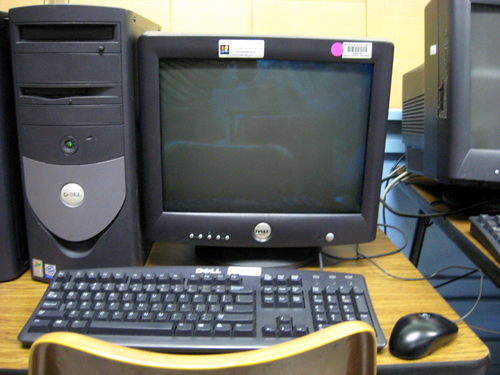
\includegraphics[width=0.18\textwidth]{gorseller/desktop.png} &
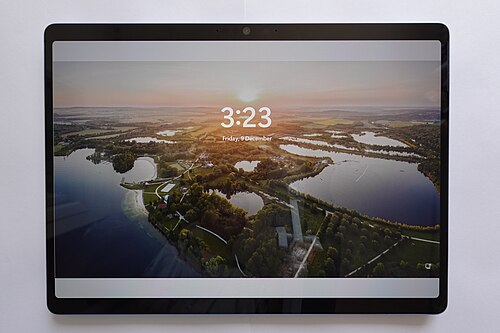
\includegraphics[width=0.18\textwidth]{gorseller/laptop.png} &
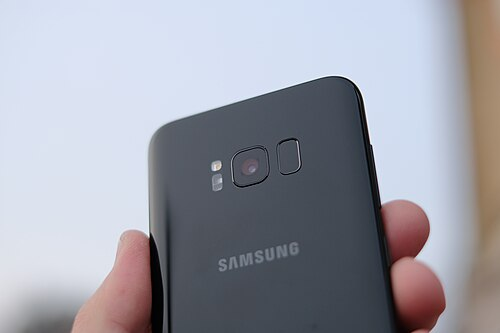
\includegraphics[width=0.18\textwidth]{gorseller/smartphone.png} &
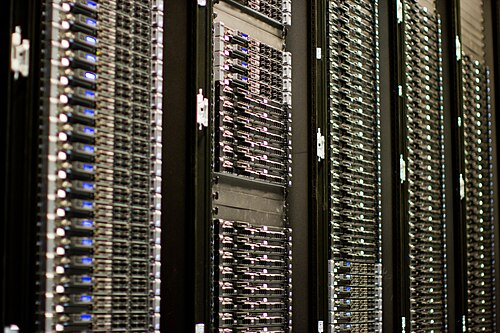
\includegraphics[width=0.18\textwidth]{gorseller/server.png} &
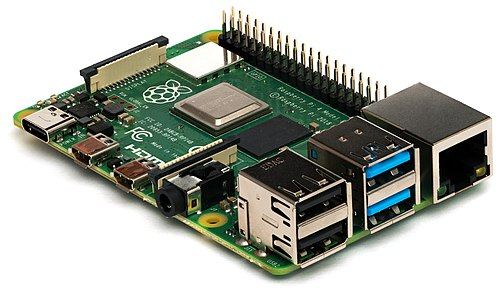
\includegraphics[width=0.18\textwidth]{gorseller/embedded.png} \\[2pt]
{\small\textbf{Masaüstü}} &
{\small\textbf{Dizüstü}} &
{\small\textbf{Akıllı Telefon}} &
{\small\textbf{Sunucu}} &
{\small\textbf{Gömülü Sistem}} \\[-1pt]
{\scriptsize\itshape Desktop} &
{\scriptsize\itshape Laptop} &
{\scriptsize\itshape Smartphone} &
{\scriptsize\itshape Server} &
{\scriptsize\itshape Embedded}
\end{tabular}
\caption{Farklı bilgisayar türleri}
\label{fig:bilgisayar-turleri}
\end{figure}


\subsection{Gerçek Dünyayla Etkileşen Bilgisayarlar}
\label{sec:fiziksel-bilgisayarlar}

Önceki alt bölümde bilgisayarın beş temel bileşenini tanıdık ve bunların masaüstünden akıllı telefona kadar çeşitli biçimlerde bir araya geldiğini gördük. Bu bileşenler yalnızca insan kullanıcıya hizmet eden aygıtlarla sınırlı değil: günümüzde giderek artan sayıda bilgisayar, gerçek dünyayı doğrudan algılayıp ona müdahale edebiliyor. İnsansı robotlar\index{insansı robot}, sürücüsüz araçlar (otonom)\index{sürücüsüz araç}\index{otonom araç}, insansız hava araçları (İHA)\index{İHA}\index{drone} ve endüstriyel robot kolları\index{endüstriyel robot} bunun en çarpıcı örnekleridir (Şekil~\ref{fig:fiziksel-bilgisayarlar}).

\begin{figure}[H]
\centering
\begin{tabular}{@{}c@{\hspace{2mm}}c@{\hspace{2mm}}c@{\hspace{2mm}}c@{}}
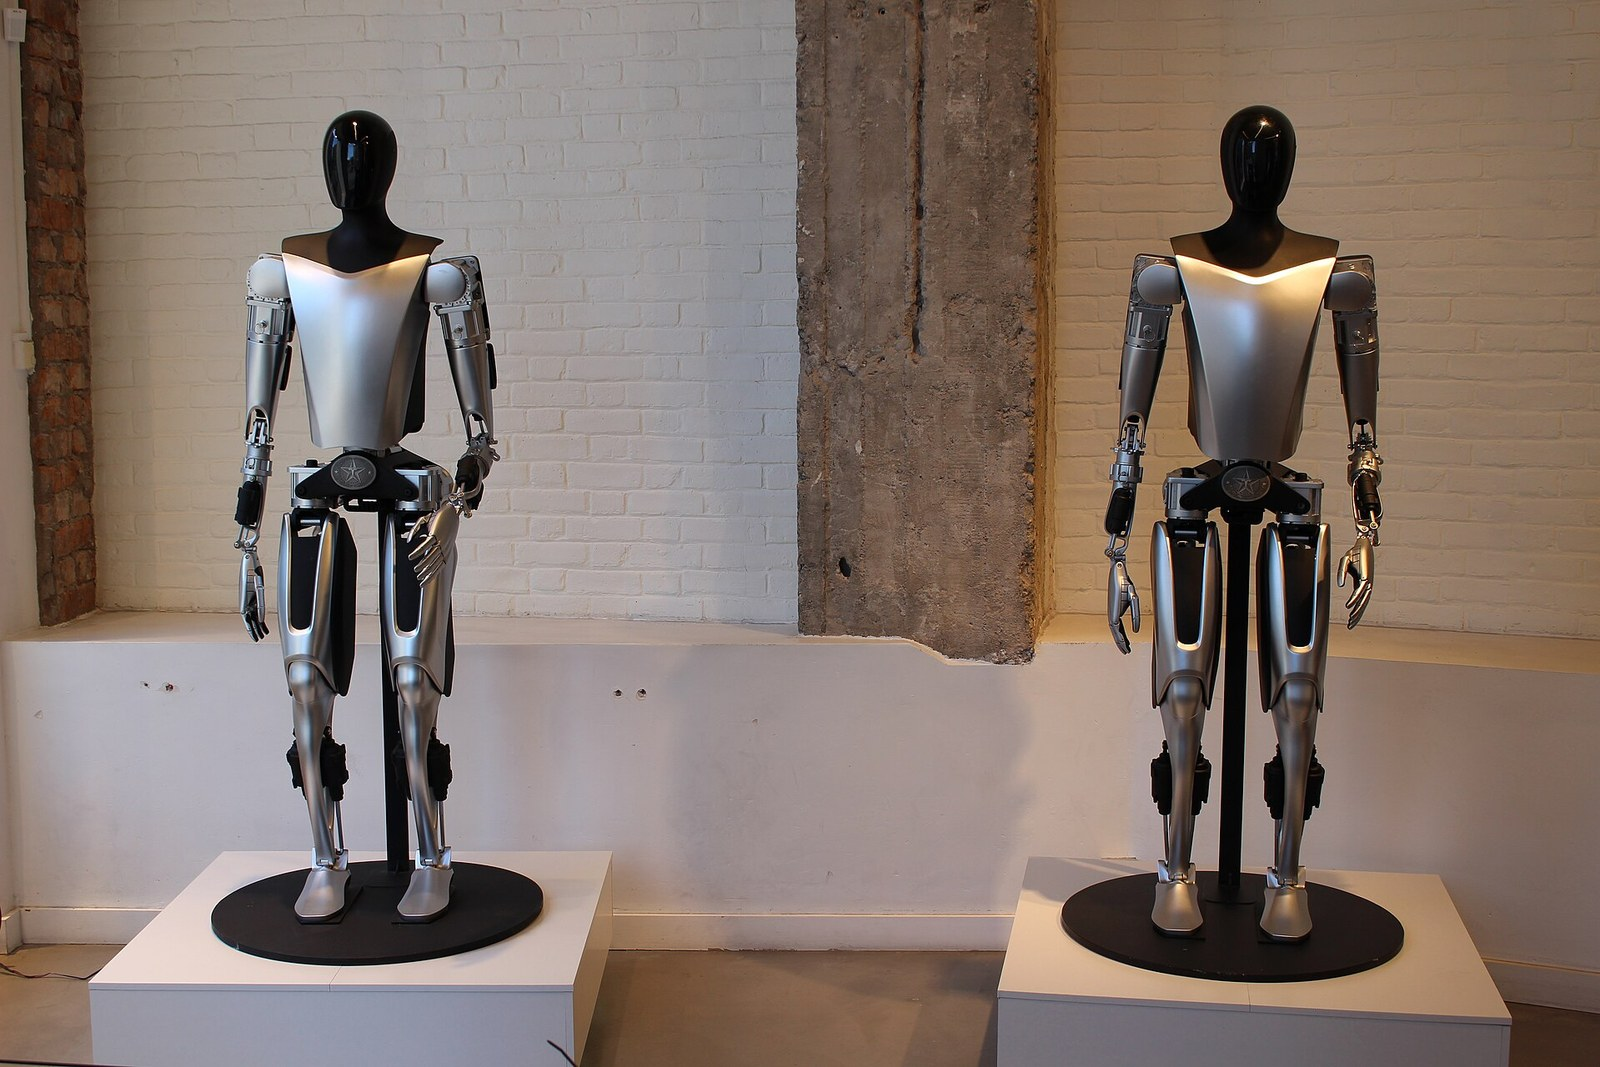
\includegraphics[width=0.23\textwidth]{gorseller/humanoid-robot.jpg} &
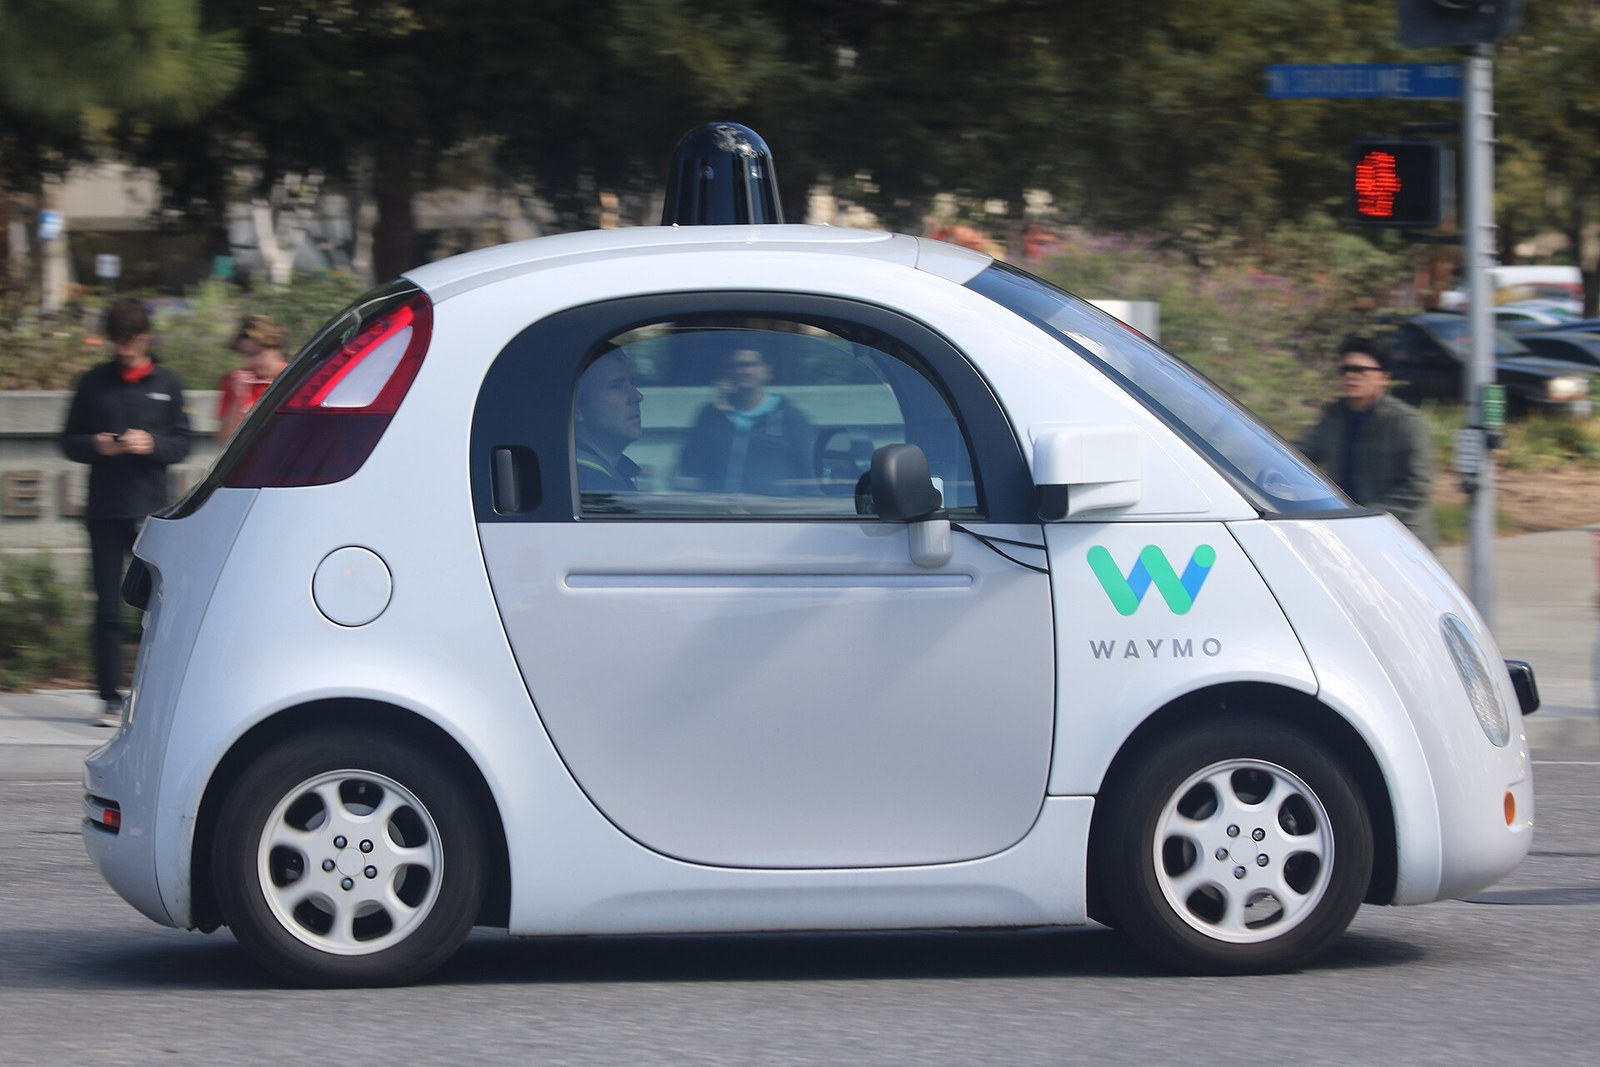
\includegraphics[width=0.23\textwidth]{gorseller/surucusuz-arac.jpg} &
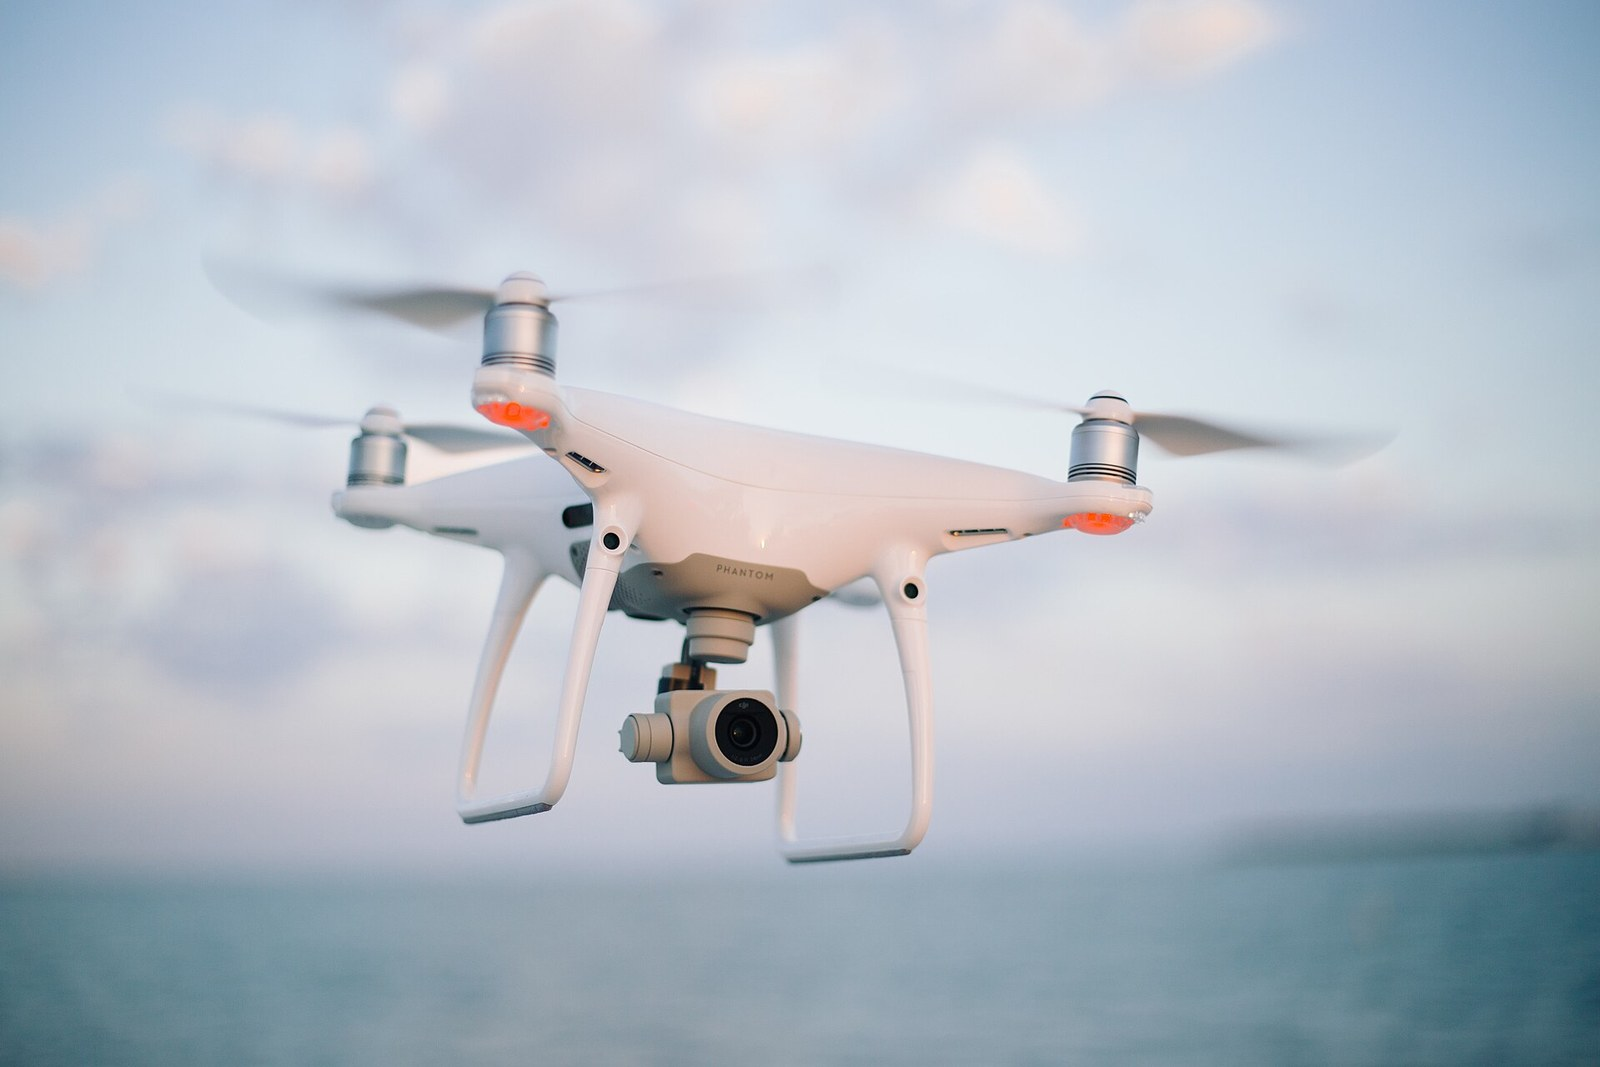
\includegraphics[width=0.23\textwidth]{gorseller/iha-drone.jpg} &
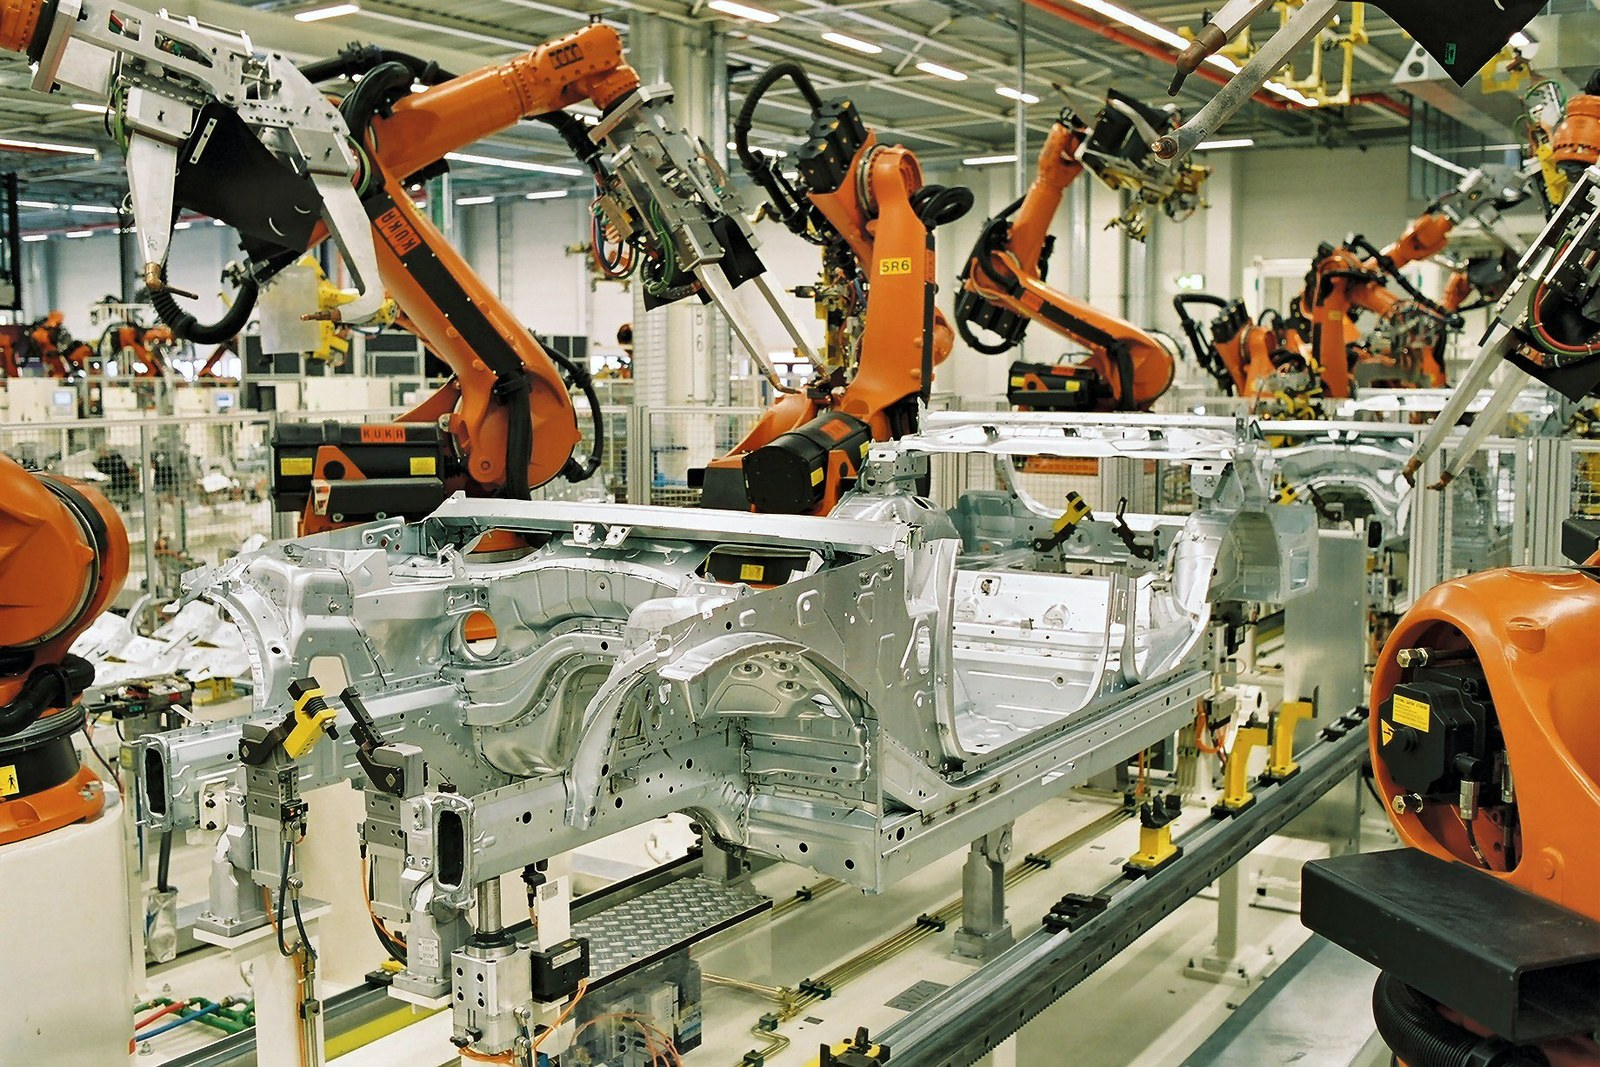
\includegraphics[width=0.23\textwidth]{gorseller/endustriyel-robot.jpg} \\[2pt]
{\small\textbf{İnsansı Robot}} &
{\small\textbf{Sürücüsüz Araç}} &
{\small\textbf{İHA (Drone)}} &
{\small\textbf{Endüstriyel Robot}} \\[-1pt]
{\scriptsize\itshape Humanoid Robot} &
{\scriptsize\itshape Autonomous Vehicle} &
{\scriptsize\itshape UAV / Drone} &
{\scriptsize\itshape Industrial Robot}
\end{tabular}
\caption{Gerçek dünyayla etkileşen bilgisayar örnekleri}
\label{fig:fiziksel-bilgisayarlar}
\end{figure}

\subsubsection*{Beş bileşen aynı, giriş/çıkış farklı}
Sayılan sistemlerin her biri özünde bir bilgisayardır ve Şekil~\ref{fig:bes-bilesen}'te gösterilen beş bileşeni eksiksiz barındırır. Onları farklı kılan şey giriş ve çıkış aygıtlarıdır. Geleneksel bir bilgisayarda giriş aygıtı klavye ve fare, çıkış aygıtı ise monitör ve hoparlördür. Oysa bir insansı robotta giriş aygıtları stereo kameralar (gözler), mikrofonlar (kulaklar), LiDAR\index{LiDAR}, kuvvet/tork algılayıcıları ve eklem konum algılayıcılarıdır. Çıkış aygıtları ise bacak ve kol eklemlerini hareket ettiren elektrik motorları ve sürücüleridir (\emph{actuator})\index{eyleyici}. Bir sürücüsüz araçta da durum farklı değildir: kameralar, radar\index{radar}, LiDAR ve ultrasonik algılayıcılar\index{ultrasonik algılayıcı} giriş sağlarken; direksiyon motoru, gaz ve fren denetleyicileri çıkış aygıtlarını oluşturur.

\subsubsection*{Gerçek zamanlılık gereksinimi}
Çevreyle etkileşen sistemlerde en önemli mimari kısıt \emph{gerçek zamanlılık}\index{gerçek zamanlı sistem} (\emph{real-time}) gereksinimidir. Bir masaüstü bilgisayarda fare tıklamasına verilen yanıtın birkaç milisaniye gecikmesi fark edilmeyebilir; ancak saatte 100\,km hızla giden bir sürücüsüz aracın çevreyi algılayıp karar vermesi için yalnızca birkaç on milisaniye süresi vardır. Bu nedenle bu tür sistemlerdeki işlemciler, saniyede milyonlarca algılayıcı verisini birleştirmeli (\emph{sensor fusion})\index{algılayıcı birleştirme}, yapay zekâ modelleriyle çevreyi yorumlamalı ve eyleyicilere komut göndermeli --- tüm bunları kesin zaman sınırları içinde yapmalıdır. Bu gereksinim, özel yapay zekâ hızlandırıcılarının (GPU, NPU, TPU gibi) bu platformlara entegre edilmesinin temel nedenidir ve Bölüm~\ref{chap:gpu-hizlandiricilar}'da ayrıntılı olarak ele alınacaktır.

\subsubsection*{Bilgisayar mimarisi açısından önemi}
Gerçek dünyayla etkileşen bilgisayarlar, mimari tasarımı birçok yönden zorlamaktadır: algılayıcılardan gelen yüksek bant genişlikli veri akışları verimli giriş/çıkış alt sistemleri gerektirir; gerçek zamanlı yapay zekâ çıkarımı güçlü paralel işlem kapasitesi talep eder; enerji kaynağının sınırlı olması (pil) düşük güç tüketimini zorunlu kılar; güvenlik açısından kritik kararların deterministik zamanda tamamlanması gerekir. Bu gereksinimler, bilgisayar mimarisinin geleceğini şekillendiren en önemli itici güçlerden biri hâline gelmiştir.


\section{İşlemci ve Yonga Üretimi}
\label{sec:islemci}

Bilgisayarın beş ana bileşeni arasında bilgisayarın kalbi sayılan \textbf{işlemci}\index{işlemci} özel bir yere sahiptir. İşlemci, bellekten okunan buyrukları yorumlayıp yürüten, aritmetik ve mantık işlemlerini gerçekleştiren ve tüm sistemi denetleyen merkezi birimdir. Bir bilgisayarın ne kadar hızlı çalışacağı, ne kadar enerji tüketeceği ve hangi iş yüklerini kaldırabileceği büyük ölçüde işlemcisinin tasarımına bağlıdır. Bu nedenle bilgisayar mimarisinin en temel konusu işlemci tasarımıdır ve bu kitabın büyük bölümü işlemcinin iç yapısını, çalışma ilkelerini ve başarımını artırma yöntemlerini ele almaktadır. Şimdi bu kritik bileşenin nasıl üretildiğini inceleyelim.

\subsection{İşlemcinin Yapılışı}
\label{sec:islemcinin-yapilisi}
İlk olarak vakum tüpleri\index{vakum tüpü} kullanılarak yapılan işlemci daha sonra transistörlerle yapılmaya başlandı. Yapısı oldukça karmaşık olan işlemcinin yapımında milyonlarca, hatta milyarlarca transistör kullanılabiliyor. Örneğin Apple M4 yongasında yaklaşık 28 milyar, AMD EPYC işlemcisinde ise 50 milyardan fazla transistör bulunur. Bu denli büyük bir karmaşıklığı yönetmek için işlemci tasarımının değişik aşamaları birbirinden soyutlanır. \emph{Soyutlama}\index{soyutlama}, her katmandaki ayrıntıları bir üst katmandan gizleyerek karmaşıklığın denetlenmesini kolaylaştırır. Örneğin bir derleyici, işlemcinin içindeki transistör bağlantılarını bilmek zorunda değildir; yalnızca buyruk kümesi düzeyindeki soyutlamayla çalışır. Benzer biçimde bir işlemci tasarımcısı, transistörlerin fiziksel üretim sürecini değil, mantık kapısı düzeyindeki davranışları temel alır.

\subsection{Tümleşik Devreler}
\label{sec:tumlesik-devreler}
Bölüm~\ref{sec:bilgisayar-gelisimi}'de anlatıldığı gibi, tümleşik devrelerin\index{tümleşik devre} keşfi bilgisayar tarihinin dönüm noktalarından biridir. Tümleşik devredeki ana fikir, transistörler, dirençler, kapasitörler ve bunlar arasındaki bağlantıların tamamının aynı yarı iletken malzeme üzerine tek bir süreçle üretilmesidir. Böylece ayrık bileşenlerden oluşan devrelere kıyasla çok daha küçük, hızlı ve güvenilir yongalar\index{yonga} elde ediliyor.

Tümleşik devreler, içerdikleri transistör sayısına göre sınıflandırılır: birkaç düzine transistör barındıran \emph{SSI}\index{SSI} (Small Scale Integration), birkaç yüz transistörlük \emph{MSI}\index{MSI}, on binlerce transistörlük \emph{LSI}\index{LSI} ve yüz binlerin üzerine çıkan \emph{VLSI}\index{VLSI} (Very Large Scale Integration --- Çok Büyük Ölçekli Tümleştirme). Günümüzdeki işlemciler milyarlarca transistör içermekte olup artık ``ultra-VLSI'' olarak nitelendirilebilecek bir ölçektedir. Transistör boyutlarının küçülmesi, aynı alana daha fazla transistör sığdırılmasını sağlamış; ancak beraberinde güç tüketimi, ısı yönetimi ve üretim maliyeti gibi yeni mühendislik zorlukları da getirmiştir.

\subsection{Yonga Üretim Süreci}
\label{sec:yonga-uretim-sureci}

\begin{figure}[ht!]
\centering
\begin{tikzpicture}[>=Stealth, scale=0.92, every node/.style={transform shape},
    adim/.style={draw, thick, rounded corners=4pt, minimum width=2.8cm,
                 minimum height=2.6cm, font=\footnotesize\bfseries, align=center,
                 inner sep=3pt}]

    % ============ ÜST SIRA (soldan sağa) ============

    % 1. Tasarım — devre şeması ikonu
    \node[adim, fill=blokmavi] (tasarim) at (0,0) {};
    \begin{scope}[shift={(tasarim.center)}, yshift=0.2cm, scale=1.3]
        \draw[thin, gray!60] (-0.6,-0.4) grid[step=0.3] (0.6,0.4);
        \draw[thick, sinyalmavi] (-0.6,-0.1) -- (-0.3,-0.1) -- (-0.3,0.2) -- (0.3,0.2) -- (0.3,-0.1) -- (0.6,-0.1);
        \fill[sinyalmavi] (-0.3,-0.1) circle (1.5pt);
        \fill[sinyalmavi] (0.3,0.2) circle (1.5pt);
    \end{scope}

    % 2. Maske Hazırlama — katmanlı dikdörtgenler
    \node[adim, fill=blokmavi] (maske) at (3.5,0) {};
    \begin{scope}[shift={(maske.center)}, yshift=0.2cm, scale=1.3]
        \fill[sinyalmavi!30] (-0.5,-0.25) rectangle (0.5,0.35);
        \fill[sinyalmavi!50, opacity=0.7] (-0.35,-0.15) rectangle (0.35,0.25);
        \draw[thick, sinyalmavi] (-0.2,0.05) rectangle (0.2,0.15);
        \draw[thick, sinyalmavi] (-0.1,-0.1) rectangle (0.4,0.0);
    \end{scope}

    % 3. Fotolitografi — UV ışınları
    \node[adim, fill=blokyesil] (isik) at (7,0) {};
    \begin{scope}[shift={(isik.center)}, yshift=0.15cm, scale=1.3]
        \fill[sinyalyesil!70!yellow] (0,0.45) circle (0.12);
        \foreach \dx in {-0.35, -0.15, 0.05, 0.25} {
            \draw[->, sinyalyesil!70!yellow, thick] (\dx+0.05,0.3) -- (\dx+0.05,-0.2);
        }
        \fill[gray!30] (-0.5,-0.25) rectangle (0.5,-0.15);
        \draw[thick] (-0.5,-0.25) rectangle (0.5,-0.15);
    \end{scope}

    % 4. Dağlama — dalgalı kimyasal çizgiler
    \node[adim, fill=blokyesil] (daglama) at (10.5,0) {};
    \begin{scope}[shift={(daglama.center)}, yshift=0.15cm, scale=1.3]
        \fill[gray!30] (-0.5,-0.3) rectangle (0.5,0.0);
        \fill[white] (-0.2,-0.05) rectangle (0.2,0.05);
        \draw[thick] (-0.5,-0.3) rectangle (0.5,0.0);
        \draw[thick] (-0.2,-0.05) -- (-0.2,0.0);
        \draw[thick] (0.2,-0.05) -- (0.2,0.0);
        \draw[sinyalkirmizi, thick, decorate, decoration={snake, amplitude=1pt, segment length=4pt}]
            (-0.4,0.2) -- (0.4,0.2);
        \draw[sinyalkirmizi, thick, decorate, decoration={snake, amplitude=1pt, segment length=4pt}]
            (-0.35,0.35) -- (0.35,0.35);
    \end{scope}

    % ============ ALT SIRA (sağdan sola) ============

    % 5. Kaplama — aşağı oklar + katman
    \node[adim, fill=bloksari] (kaplama) at (10.5,-3.8) {};
    \begin{scope}[shift={(kaplama.center)}, yshift=0.15cm, scale=1.3]
        \foreach \dx in {-0.3, -0.1, 0.1, 0.3} {
            \draw[->, thick, sinyalmavi!70!black] (\dx,0.35) -- (\dx,-0.05);
        }
        \fill[gray!25] (-0.5,-0.3) rectangle (0.5,-0.2);
        \fill[sinyalmavi!25] (-0.5,-0.2) rectangle (0.5,-0.1);
        \draw[thick] (-0.5,-0.3) rectangle (0.5,-0.1);
    \end{scope}

    % 6. Test — onay işareti
    \node[adim, fill=bloksari] (test) at (7,-3.8) {};
    \begin{scope}[shift={(test.center)}, yshift=0.1cm, scale=1.3]
        \draw[very thick, sinyalyesil] (-0.2,0.0) -- (-0.05,-0.2) -- (0.3,0.3);
        \draw[thick, gray!60] (0,0) circle (0.45);
    \end{scope}

    % 7. Kesim — plaka + testere çizgisi
    \node[adim, fill=blokkirmizi] (kesim) at (3.5,-3.8) {};
    \begin{scope}[shift={(kesim.center)}, yshift=0.1cm, scale=1.3]
        \draw[thick, fill=gray!15] (0,0) circle (0.4);
        \draw[densely dashed, sinyalkirmizi, thin] (-0.35,0.13) -- (0.35,0.13);
        \draw[densely dashed, sinyalkirmizi, thin] (-0.35,-0.13) -- (0.35,-0.13);
        \draw[densely dashed, sinyalkirmizi, thin] (-0.13,-0.35) -- (-0.13,0.35);
        \draw[densely dashed, sinyalkirmizi, thin] (0.13,-0.35) -- (0.13,0.35);
    \end{scope}

    % 8. Paketleme — yonga + pinler
    \node[adim, fill=blokkirmizi-acik] (paket) at (0,-3.8) {};
    \begin{scope}[shift={(paket.center)}, yshift=0.1cm, scale=1.3]
        \fill[gray!40] (-0.3,-0.2) rectangle (0.3,0.2);
        \draw[thick] (-0.3,-0.2) rectangle (0.3,0.2);
        \fill[sinyalmavi!30] (-0.12,-0.08) rectangle (0.12,0.08);
        \foreach \px in {-0.2, -0.05, 0.1, 0.25} {
            \draw[thick] (\px,0.2) -- (\px,0.35);
        }
        \foreach \px in {-0.2, -0.05, 0.1, 0.25} {
            \draw[thick] (\px,-0.2) -- (\px,-0.35);
        }
        \foreach \py in {-0.1, 0.1} {
            \draw[thick] (-0.3,\py) -- (-0.45,\py);
        }
        \foreach \py in {-0.1, 0.1} {
            \draw[thick] (0.3,\py) -- (0.45,\py);
        }
    \end{scope}

    % ============ OKLAR (kesikli çizgiden önce çiz) ============

    % Üst sıra (soldan sağa)
    \draw[->, very thick, sinyalmavi!70!black] (tasarim.east) -- (maske.west);
    \draw[->, very thick, sinyalmavi!70!black] (maske.east) -- (isik.west);
    \draw[->, very thick, sinyalmavi!70!black] (isik.east) -- (daglama.west);

    % Aşağı dönüş (sağ taraftan geçir)
    \draw[->, very thick, sinyalmavi!70!black]
        (daglama.east) -- ++(0.8,0) |- (kaplama.east);

    % Alt sıra (sağdan sola)
    \draw[->, very thick, sinyalmavi!70!black] (kaplama.west) -- (test.east);
    \draw[->, very thick, sinyalmavi!70!black] (test.west) -- (kesim.east);
    \draw[->, very thick, sinyalmavi!70!black] (kesim.west) -- (paket.east);

    % ============ KESİKLİ ÇERÇEVE (okların üstüne, etiketlerin altına) ============
    \draw[dashed, thick, gray!50, rounded corners=5pt]
        ([xshift=-0.5cm, yshift=0.7cm]isik.north west) rectangle
        ([xshift=1.15cm, yshift=-0.7cm]kaplama.south east);

    % ============ ETİKETLER VE NUMARALAR (en üste — kesikli çizginin üstünde) ============
    \node[font=\footnotesize\bfseries, anchor=north] at ([yshift=-0.05cm]tasarim.south) {Tasarım};
    \node[font=\footnotesize\bfseries, fill=white, inner sep=1pt, text=gray!50!black] at ([yshift=0.2cm]tasarim.north) {1};

    \node[font=\footnotesize\bfseries, anchor=north] at ([yshift=-0.05cm]maske.south) {Maske};
    \node[font=\footnotesize\bfseries, fill=white, inner sep=1pt, text=gray!50!black] at ([yshift=0.2cm]maske.north) {2};

    \node[font=\footnotesize\bfseries, anchor=north] at ([yshift=-0.05cm]isik.south) {Fotolitografi};
    \node[font=\footnotesize\bfseries, fill=white, inner sep=1pt, text=gray!50!black] at ([yshift=0.2cm]isik.north) {3};

    \node[font=\footnotesize\bfseries, anchor=north] at ([yshift=-0.05cm]daglama.south) {Dağlama};
    \node[font=\footnotesize\bfseries, fill=white, inner sep=1pt, text=gray!50!black] at ([yshift=0.2cm]daglama.north) {4};

    \node[font=\footnotesize\bfseries, anchor=north] at ([yshift=-0.05cm]kaplama.south) {Kaplama};
    \node[font=\footnotesize\bfseries, fill=white, inner sep=1pt, text=gray!50!black] at ([yshift=0.2cm]kaplama.north) {5};

    \node[font=\footnotesize\bfseries, anchor=north] at ([yshift=-0.05cm]test.south) {Test};
    \node[font=\footnotesize\bfseries, fill=white, inner sep=1pt, text=gray!50!black] at ([yshift=0.2cm]test.north) {6};

    \node[font=\footnotesize\bfseries, anchor=north] at ([yshift=-0.05cm]kesim.south) {Kesim};
    \node[font=\footnotesize\bfseries, fill=white, inner sep=1pt, text=gray!50!black] at ([yshift=0.2cm]kesim.north) {7};

    \node[font=\footnotesize\bfseries, anchor=north] at ([yshift=-0.05cm]paket.south) {Paketleme};
    \node[font=\footnotesize\bfseries, fill=white, inner sep=1pt, text=gray!50!black] at ([yshift=0.2cm]paket.north) {8};

    % Tekrarlama notu (en üstte)
    \node[font=\scriptsize\itshape, fill=white, inner sep=2pt, text=gray!40!black, anchor=south] at (8.75,1.8)
        {Bu adımlar 50+ katman için tekrarlanır};

\end{tikzpicture}
\caption[Yonga yapılma süreci]{Yonga yapılma süreci. Modern bir işlemcinin üretiminde fotolitografi--dağlama--kaplama adımları onlarca katman için tekrarlanır.}
\label{fig:yonga-yapim}
\end{figure}

Yapılması planlanan yonga öncelikle bilgisayar üzerinde plan olarak çizilir ve denenir. Işıklı baskı (photolithography) tekniğiyle tüm yongaların basılması için bir kalıp hazırlanır. Silisyum\index{silisyum} silindirden kristal bir testereyle kesilen ince katmanların üzerine katmanları birbirinden yalıtacak şekilde silisyum oksit kaplanır ve kalıbın ana hatlarının geçilebilmesi için ışığa duyarlı bir tabaka kaplanır. Yonga yapım süreci Şekil~\ref{fig:yonga-yapim}'te gösterilmiştir.

\begin{bilginot}[Silisyum mu, Silikon mu?]
Yarı iletken yongaların temel malzemesi olan kimyasal element İngilizcede \emph{silicon} (Si, atom numarası~14), Türkçede ise \textbf{silisyum} olarak adlandırılır. Günlük dilde sıkça karşılaşılan ``silikon'' sözcüğü ise İngilizce \emph{silicone} kelimesinin karşılığıdır ve silisyum ile oksijenden türetilmiş sentetik bir polimeri ifade eder (mutfak kalıpları, conta malzemeleri vb.). Dolayısıyla yonga üretiminde kullanılan malzeme \emph{silisyum}, ABD'deki ünlü teknoloji vadisinin adı ise doğru çevirisiyle \emph{Silisyum Vadisi}'dir.
\end{bilginot}

\begin{figure}[ht!]
\centering
\begin{tikzpicture}[>=Stealth]
    \def\R{3.8}        % plaka yarıçapı
    \def\ks{0.7}       % kırmık kenar uzunluğu
    \def\kg{0.08}      % kırmıklar arası boşluk (kesim payı)
    \def\adim{0.78}    % ızgara adımı = ks + kg
    \def\ha{0.35}      % yonga yarı kenarı = ks/2

    % --- 1. Silisyum plaka (arka plan) ---
    \fill[gray!12] (0,0) circle (\R);
    \begin{scope}
        \clip (0,0) circle (\R);
        \fill[white] (-0.4,{-\R-0.1}) rectangle (0.4,{-\R+0.25});
    \end{scope}

    % --- 2. Kırmık ızgarası (sadece dört köşesi de dairenin içinde olanlar) ---
    \foreach \i in {-5,-4,...,5} {
        \foreach \j in {-5,-4,...,5} {
            \pgfmathsetmacro{\cx}{\i*\adim}
            \pgfmathsetmacro{\cy}{\j*\adim}
            \pgfmathsetmacro{\da}{sqrt((\cx-\ha)^2+(\cy-\ha)^2)}
            \pgfmathsetmacro{\db}{sqrt((\cx+\ha)^2+(\cy-\ha)^2)}
            \pgfmathsetmacro{\dc}{sqrt((\cx+\ha)^2+(\cy+\ha)^2)}
            \pgfmathsetmacro{\dd}{sqrt((\cx-\ha)^2+(\cy+\ha)^2)}
            \pgfmathsetmacro{\dmax}{max(\da,max(\db,max(\dc,\dd)))}
            \pgfmathparse{\dmax < (\R-0.15) ? 1 : 0}
            \ifnum\pgfmathresult=1
                \fill[sinyalmavi!12] ({\cx-\ha},{\cy-\ha}) rectangle ({\cx+\ha},{\cy+\ha});
                \draw[gray!40, thin] ({\cx-\ha},{\cy-\ha}) rectangle ({\cx+\ha},{\cy+\ha});
            \fi
        }
    }

    % --- 3. Kenar yongaları (kısmi, verim kaybı göstermek için) ---
    \begin{scope}
        \clip (0,0) circle ({\R-0.05});
        \foreach \i in {-5,-4,...,5} {
            \foreach \j in {-5,-4,...,5} {
                \pgfmathsetmacro{\cx}{\i*\adim}
                \pgfmathsetmacro{\cy}{\j*\adim}
                \pgfmathsetmacro{\da}{sqrt((\cx-\ha)^2+(\cy-\ha)^2)}
                \pgfmathsetmacro{\db}{sqrt((\cx+\ha)^2+(\cy-\ha)^2)}
                \pgfmathsetmacro{\dc}{sqrt((\cx+\ha)^2+(\cy+\ha)^2)}
                \pgfmathsetmacro{\dd}{sqrt((\cx-\ha)^2+(\cy+\ha)^2)}
                \pgfmathsetmacro{\dmax}{max(\da,max(\db,max(\dc,\dd)))}
                \pgfmathsetmacro{\dmin}{sqrt(\cx*\cx+\cy*\cy)}
                \pgfmathparse{(\dmax >= (\R-0.15)) && (\dmin < (\R-0.3)) ? 1 : 0}
                \ifnum\pgfmathresult=1
                    \fill[gray!8] ({\cx-\ha},{\cy-\ha}) rectangle ({\cx+\ha},{\cy+\ha});
                    \draw[gray!25, thin, densely dashed] ({\cx-\ha},{\cy-\ha}) rectangle ({\cx+\ha},{\cy+\ha});
                \fi
            }
        }
    \end{scope}

    % --- 4. Plaka konturu (üstte, temiz kenar) ---
    \draw[thick, gray!70] (0,0) circle (\R);
    % Çentik (notch)
    \draw[thick, gray!70] ({-0.35},{-sqrt(\R*\R-0.35*0.35)})
        -- (0,{-\R+0.2})
        -- ({0.35},{-sqrt(\R*\R-0.35*0.35)});

    % --- 5. Bir yongayı vurgula ---
    \draw[very thick, sinyalyesil, fill=sinyalyesil!15]
        ({-\ha},{\adim-\ha}) rectangle ({\ha},{\adim+\ha});

    % --- 6. Etiketler (sağ tarafta, düzenli) ---
    % Kırmık etiketi
    \draw[->, thick, sinyalyesil!70!black] (4.8,2.8) -- (0.45,1.1);
    \node[font=\footnotesize, anchor=west] at (4.9,2.8) {Kırmık (\textit{die})};

    % Hatalı kırmık etiketi (kenar)
    \draw[->, thick, gray!50] (4.8,1.2) -- (3.12,1.56);
    \node[font=\footnotesize, text=gray!60!black, anchor=west] at (4.9,1.4) {Kullanılamayan};
    \node[font=\footnotesize, text=gray!60!black, anchor=west] at (4.9,1.0) {kenar kırmık};

    % Çentik etiketi
    \draw[->, thick, gray!50] (1.8,-4.3) -- (0.15,{-\R+0.22});
    \node[font=\footnotesize, text=gray!60!black, anchor=west] at (1.9,-4.3) {Çentik (\textit{notch})};

    % --- 7. Alt bilgiler ---
    \node[font=\footnotesize\itshape, text=gray!60!black] at (0,-5.0)
        {Silisyum plaka (\textit{wafer})};

    % Çap göstergesi
    \draw[<->, thick, gray!50!black] (-\R,-4.5) -- (\R,-4.5);
    \node[font=\footnotesize, fill=white, inner sep=1pt] at (0,-4.5) {$\varnothing$ 300\,mm};

\end{tikzpicture}
\caption{Bir silisyum plakadan yongaların kesilmesi}
\label{fig:silisyum-plaka}
\end{figure}

\begin{bilginot}[Silisyum plaka neden yuvarlak?]
Öğrenciler sıklıkla ``Plaka neden kare değil, kare olsa daha fazla kırmık sığmaz mı?'' diye sorar. Yanıt üretim sürecinde yatmaktadır. Silisyum plakalar \emph{Czochralski yöntemi}\index{Czochralski yöntemi} ile üretilir: çok saf silisyum bir potada eritilir, dönen bir tohum kristal erimiş silisyuma dokundurularak yavaşça yukarı çekilir. Dönerek çekilme hareketi doğal olarak silindirik bir tek kristal kütle (\emph{ingot}) oluşturur; bu silindirin enine kesitleri daire biçimindedir. Kare plaka üretmek istendiğinde silindirik kütleden kesim sırasında büyük miktarda malzeme israf olurdu. Ayrıca yüksek sıcaklıklı üretim aşamalarında (900--1100\,°C) kare plakanın köşelerinde gerilim yoğunlaşması oluşarak kırılma riski artardı. Yuvarlak geometri ise termal genleşme sırasında gerilimi eşit biçimde dağıtır.
\end{bilginot}


\subsection{Teknoloji Düğümleri ve Gelişimi}
\label{sec:teknoloji-dugumleri}

Bir yonga üretim sürecinin en temel parametresi \emph{teknoloji düğümü}\index{teknoloji düğümü} (\emph{technology node}) olarak adlandırılan ve nanometre (nm) cinsinden ifade edilen boyuttur. Tarihsel olarak bu değer transistörün kapı uzunluğuna karşılık gelirdi; ancak günümüzde gerçek fiziksel boyutlarla doğrudan ilişkisi zayıflamış ve daha çok bir nesil göstergesi hâline gelmiştir. Her yeni teknoloji düğümüne geçişte transistör yoğunluğu yaklaşık iki katına çıkar, bu da aynı alana daha fazla transistör sığdırılmasını sağlar.

\begin{table}[ht!]
\centering
\caption[Teknoloji düğümlerinin gelişimi]{Yıllar içinde teknoloji düğümlerinin gelişimi. Transistör yoğunlukları yaklaşık değerler olup üretim tesisine ve tasarıma göre değişir.}
\label{tab:teknoloji-dugumleri}
\footnotesize
\begin{tabular}{rrrll}
\toprule
\textbf{Düğüm} & \textbf{Yıl} & \textbf{Yoğunluk (MTr/mm$^2$)} & \textbf{Öncü Üretici} & \textbf{Örnek Yonga} \\
\midrule
90\,nm   & 2004 & ${\sim}$15   & Intel     & Pentium 4 Prescott \\
65\,nm   & 2006 & ${\sim}$30   & Intel     & Core 2 Duo \\
45\,nm   & 2008 & ${\sim}$60   & Intel     & Core i7 (Nehalem) \\
32\,nm   & 2010 & ${\sim}$90   & Intel     & Sandy Bridge \\
22\,nm   & 2012 & ${\sim}$160  & Intel     & Ivy Bridge (FinFET) \\
14\,nm   & 2014 & ${\sim}$310  & Intel, Samsung & Skylake, Exynos 7 \\
10\,nm   & 2017 & ${\sim}$530  & TSMC      & Apple A11 \\
7\,nm    & 2018 & ${\sim}$910  & TSMC      & Apple A12, AMD Zen 2 \\
5\,nm    & 2020 & ${\sim}$1\,710 & TSMC    & Apple M1, A14 Bionic \\
3\,nm    & 2022 & ${\sim}$3\,000 & TSMC, Samsung & Apple M3, A17 Pro \\
\bottomrule
\end{tabular}
\end{table}

Tablo~\ref{tab:teknoloji-dugumleri}'den görüldüğü üzere, 2004'ten 2022'ye kadar transistör yoğunluğu yaklaşık 200 kat artmıştır. Ancak bu kazanımlar bedelsiz değildir: teknoloji düğümü küçüldükçe hem plaka maliyeti hem de \emph{maske seti}\index{maske seti} (\emph{mask set}) maliyeti dramatik biçimde artar. Maske seti, yonga üzerindeki her bir katmanın desenini plakaya aktarmak için kullanılan fotolitografi kalıplarının tamamıdır; modern bir işlemcide 80'den fazla maske katmanı bulunabilir ve her maske yüksek hassasiyette üretilmek zorundadır. Tablo~\ref{tab:plaka-maliyetleri} bu maliyet artışını göstermektedir.

\begin{table}[ht!]
\centering
\caption[Teknoloji düğümlerine göre üretim maliyetleri]{Farklı teknoloji düğümlerinde 300\,mm silisyum plakanın ve maske setinin yaklaşık maliyeti. Maliyetler yonga üretim tesisine ve sipariş hacmine göre değişkenlik gösterir.}
\label{tab:plaka-maliyetleri}
\footnotesize
\begin{tabular}{lrrl}
\toprule
\textbf{Düğüm} & \textbf{Plaka Maliyeti (\$)} & \textbf{Maske Seti (\$)} & \textbf{Tipik Kullanım Alanı} \\
\midrule
28\,nm    & 3\,000--4\,000     & ${\sim}$5\,M    & IoT, otomotiv, gömülü \\
16/14\,nm & 5\,000--6\,000     & ${\sim}$15\,M   & Orta seviye mobil, ağ \\
7\,nm     & 9\,000--10\,000    & ${\sim}$30\,M   & Üst seviye mobil, GPU \\
5\,nm     & 16\,000--17\,000   & ${\sim}$50\,M   & En üst düzey işlemciler \\
3\,nm     & 20\,000+           & ${\sim}$75\,M   & Son nesil yongalar \\
\bottomrule
\multicolumn{4}{l}{\scriptsize M\,=\,milyon; maliyetler tahmini olup üretim tesisine ve hacme göre değişir.}
\end{tabular}
\end{table}

3\,nm düğümünde bir maske setinin maliyeti 75 milyon doları aşabilmektedir. Bu durum, ileri düğümlerde üretimi yalnızca çok yüksek hacimli ürünler (akıllı telefon işlemcileri, veri merkezi yongaları) için ekonomik kılar. Düşük hacimli uygulamalar --- IoT algılayıcıları, otomotiv denetleyicileri gibi --- maliyet açısından 28\,nm veya 16\,nm gibi olgun düğümlerde üretilmeye devam eder. Bu ekonomik gerçeklik, farklı uygulama alanlarının farklı teknoloji düğümlerinde kalmasına neden olur ve ``en yeni teknoloji her zaman en iyi seçimdir'' yanılgısını çürütür.


\subsection{Üretim Maliyeti ve Verim}
\label{sec:maliyet-verim}

Yonga üretiminin ekonomisini anlamak, mimari kararlar için kritiktir. Büyük alanlı yongalar daha fazla transistör barındırabilir ancak verim düşüşü nedeniyle orantısız biçimde pahalılaşır. Tasarımcılar yonga alanı, üretim maliyeti ve verim arasındaki dengeyi gözetmek zorundadır.

Bir yonganın üretim maliyeti aşağıdaki denklemle gösterilebilir:
\begin{equation}
\text{Yonga maliyeti} = \frac{\text{Plaka maliyeti}}{\text{Plakadaki yonga sayısı} \times \text{Verim}}
\label{eq:yonga-maliyet}
\end{equation}

Plakanın alacağı yonga sayısı yaklaşık olarak aşağıdaki eşitlikle gösterilebilir:
\begin{equation}
\text{Plakadaki yonga sayısı} = \frac{\text{Plaka alanı}}{\text{Yonga alanı}}
\label{eq:yonga-sayisi}
\end{equation}

Verim yaklaşık olarak aşağıdaki denklemle modellenir:
\begin{equation}
\text{Verim} = \left( \frac{1}{1 + \text{Birim alan başına hata sayısı} \times \text{Yonga alanı}} \right)^{N}
\label{eq:verim}
\end{equation}
Bu denklemdeki kesirin paydasındaki değerin üssü ($N$) üretim sürecindeki kritik aşama sayısı ile ilişkilidir.

\subsubsection*{Verim Öğrenme Eğrisi}

Yeni bir teknoloji düğümü üretime girdiğinde verim genellikle düşüktür --- tipik olarak \%30--50 arasında başlar. Üretim süreci olgunlaştıkça ve hata kaynakları belirlendikçe verim kademeli olarak \%80--90 ve üzerine çıkar. Bu iyileşme sürecine \emph{verim öğrenme eğrisi}\index{verim öğrenme eğrisi} (\emph{yield learning curve}) denir ve bir yonga üretim tesisinin teknolojik olgunluğunun en önemli göstergesidir.

Verim verisi şirketler tarafından ticari sır olarak korunduğundan kesin rakamlar kamuya açıklanmaz; ancak genel eğilimler endüstri analistleri tarafından raporlanır. Örneğin TSMC'nin 7\,nm süreci (N7) 2018'de üretime girdiğinde verimlerin birkaç çeyrek dönem içinde \%80'in üzerine çıktığı tahmin edilmektedir. Denklem~\ref{eq:yonga-maliyet}'ten görüldüğü üzere verim yarıya düşerse yonga maliyeti iki katına çıkar; bu nedenle yonga üreticileri yeni düğümlerde verimi artırmak için büyük mühendislik yatırımları yapar.

\begin{ornek}[1.1]
Bir yonga tasarım şirketi, akıllı telefon işlemcisi için 3\,nm teknolojisini kullanmayı düşünüyor. Yonganın kırmık alanı 100\,mm$^2$ olacak. 300\,mm çaplı bir plakanın maliyeti 20\,000\,\$, maske setinin maliyeti 75\,M\,\$, olgun süreçteki verim \%75 olsun. Bir kırmığın üretim maliyetini ve maske seti payını iki farklı üretim hacmi için hesaplayın: (a)~100 milyon adet, (b)~1 milyon adet.

\textbf{Çözüm:}\\
Plaka alanı: $A_\text{plaka} = \pi \times 150^2 \approx 70\,686$\,mm$^2$.

Plakadaki kırmık sayısı (yaklaşık): $70\,686 \div 100 \approx 706$ kırmık. Kenar kayıpları düşüldüğünde kullanılabilir kırmık sayısı yaklaşık 600'dür.

Verimli kırmık sayısı: $600 \times 0{,}75 = 450$ iyi kırmık/plaka.

Plaka başına kırmık maliyeti (Denklem~\ref{eq:yonga-maliyet}): $20\,000 \div 450 \approx 44{,}4$\,\$/kırmık.

\medskip
\textbf{Maske seti payı:}

\smallskip
\begin{tabular}{@{}lrl@{}}
100 milyon adet: & $75\,000\,000 \div 100\,000\,000 = 0{,}75$\,\$/kırmık & $\Rightarrow$ \textbf{toplam $\approx$ 45\,\$/kırmık} \\[4pt]
1 milyon adet:   & $75\,000\,000 \div 1\,000\,000 = 75$\,\$/kırmık     & $\Rightarrow$ \textbf{toplam $\approx$ 119\,\$/kırmık}
\end{tabular}

\medskip
\textbf{Karşılaştırma:} Aynı yonga 28\,nm'de üretilseydi plaka maliyeti ${\sim}$3\,500\,\$, maske seti ${\sim}$5\,M\,\$, verim ${\sim}$\%90 olacaktı. Plaka başına maliyet ${\sim}$6{,}5\,\$/kırmık, 1 milyon adet için maske payı 5\,\$/kırmık, toplam ${\sim}$11{,}5\,\$/kırmık --- 3\,nm'dekinin onda biri. Ancak 28\,nm'de aynı alana sığan transistör sayısı 3\,nm'nin yüzde biri kadar olduğundan, aynı işlevsellik çok daha büyük bir kırmık alanı gerektirir.

Bu örnek, ileri teknoloji düğümlerinin neden yalnızca yüksek hacimli ürünlerde ekonomik olduğunu ve maske seti maliyetinin düşük hacimlerde baskın hâle geldiğini göstermektedir.
\end{ornek}

\begin{ornek}[1.2]
Çapı 300\,mm olan bir silisyum plakanın maliyeti 12\,000\,\$ olsun. Üretilecek yonganın alanı 200\,mm$^2$, birim alan başına hata sayısı 0{,}03\,hata/mm$^2$ ve kritik aşama sayısı $N=12$ ise bir yonganın maliyetini hesaplayın.

\textbf{Çözüm:}\\
Plaka alanı: $A_\text{plaka} = \pi \times 150^2 \approx 70\,686$\,mm$^2$.

Plakadaki yonga sayısı: $\displaystyle\frac{70\,686}{200} \approx 353$ yonga.

Verim: $\displaystyle\left(\frac{1}{1 + 0{,}03 \times 200}\right)^{12} = \left(\frac{1}{7}\right)^{12} \approx 7{,}3 \times 10^{-11}$ --- bu son derece düşük bir verimdir!

Gerçek üretimde birim alan başına hata sayısı çok daha düşüktür. Eğer hata yoğunluğu 0{,}001\,hata/mm$^2$ olsaydı:
\[
\text{Verim} = \left(\frac{1}{1 + 0{,}001 \times 200}\right)^{12} = \left(\frac{1}{1{,}2}\right)^{12} \approx 0{,}112
\]
Bu durumda yonga maliyeti: $\displaystyle\frac{12\,000}{353 \times 0{,}112} \approx 303$\,\$.

Bu örnek, yonga alanının ve hata yoğunluğunun maliyet üzerindeki dramatik etkisini açıkça gösteriyor.
\end{ornek}


\section{Programların Çalıştırılması}
\label{sec:program-calistirma}

Bilgisayarın donanım bileşenlerini ve işlemcinin yapısını tanıdığımıza göre, şimdi bir programın bu donanım üzerinde nasıl çalıştığına bakalım. Bir programı makine üzerinde çalıştırmak için öncelikle makineyle aynı dilin konuşulması gerekir. Bilgisayarların alfabesi 1'ler ve 0'lardan oluşur; bu alfabedeki harflerden oluşan sözcükler ise ikilik tabanda yazılmış sayılardır. Sözcüklerdeki 1 ya da 0 rakamlarından oluşan her bir basamağa ``Binary Digit'' veya kısaca ``Bit''\index{bit} denir. Bilgisayarların anladığı kelimeler 1 ve 0'lardan oluştuğu için üst düzey dilde yazılanların bilgisayar tarafından anlaşılması bunların ikilik düzene çevrilmesiyle mümkün olur. Yazılan kodlar makinenin anlayabileceği sayılara buyruklar sayesinde çevriliyor.

Önceleri bütün işlemler doğrudan makine dili\index{makine dili} kullanılarak yapılıyordu. Daha sonra insan mantığına ve konuşma biçimine uygun yollar geliştirildi. Komutlar yalnızca sayılarla değil, kelimeler kullanılarak da bilgisayara iletildi. Bilgisayarlara emir vermek için ikilik tabandaki sayılar yerine küçük anlamlı sözcükler kullanan bu dillere \emph{çevirici dil}\index{çevirici dil} (\emph{Assembly}) denir. Makine kodlarına en yakın kod çevirici dil kodudur. Bu kod, yazıldıktan sonra makine üzerinde kurulmuş çeviricilerle (\emph{Assembler}) tekrar makine diline dönüştürülür. Örneğin çevirici dilde \texttt{add A, B, C} yazıldığında, çevirici program bu kodu \texttt{10001010101010101100010000100010} olarak makine diline çevirir.

Buyrukların saklanma şekilleri de mimari tasarımda temel sorunlardan biri haline geldi ve bunun çözümü için farklı mimariler geliştirildi. Bu mimarilerden birisi pek çok tasarımın temelini oluşturacak yapıyı kuran Von Neumann'ın\index{Von Neumann mimarisi} tasarladığı mimaridir. Buyruklar ve verilerin aynı bellekte saklandığı bu tasarımda aynı anda hem buyruk hem de veri ile işlem yapılmaya çalışıldığında belleğe erişim bir darboğaz oluşturabiliyor. Buna \emph{Von Neumann darboğazı}\index{Von Neumann darboğazı} denir. Darboğaz sorununu ortadan kaldırmayı amaçlayan bir diğer mimari tasarım yöntemi de buyrukların ve verilerin farklı belleklerde saklandığı \emph{Harvard mimarisi}\index{Harvard mimarisi}dir.

Buyrukların tasarımı için iki temel gerçekleştirme yöntemi söz konusu. Birincisi her bir buyruğun temel ve yalın işlemleri ifade ettiği RISC\index{RISC} (\emph{Reduced Instruction Set Computer} --- İndirgenmiş Buyruk Kümeli Bilgisayar), diğeri de buyrukların karmaşık işlemleri gerçekleştirecek şekilde tasarlandığı CISC\index{CISC} (\emph{Complex Instruction Set Computer} --- Karmaşık Buyruk Kümeli Bilgisayar) mimarisidir. Örneğin RISC için yazılan üç buyruğun yaptığı işi CISC tasarımlarında bir buyruk yapabiliyor. Ancak bu durumda CISC'in kullanımı kolay, devre düzeyinde gerçekleştirmesi zor ve karmaşık. Tam tersi olarak RISC'te ise buyrukları devre düzeyinde gerçekleştirmek kolay, ancak yalın buyruklarla kodlama yapmak daha zor ve bu buyruklarla yazılan programların kod satırı sayısı CISC mimarisine göre daha fazla.

\begin{bilginot}[RISC-V: Bu Kitabın Buyruk Kümesi]
Bu kitapta buyruk kümesi mimarisi olarak açık kaynaklı \textbf{RISC-V}\index{RISC-V} kullanılıyor. RISC-V'nin neden tercih edildiği, tescilli mimarilerle karşılaştırması ve endüstrideki yeri Bölüm~\ref{sec:neden-riscv}'de ayrıntılı olarak ele alınıyor.
\end{bilginot}

\begin{figure}[H]
\centering
\begin{tikzpicture}[>=Stealth, node distance=1.8cm]
    % Üst düzey program kutusu
    \node[blok, fill=blokyesil, minimum width=7cm, minimum height=1.4cm] (ust)
        {\textbf{Üst Düzey Program}\\[2pt]\texttt{A = B + C;}};

    % Derleyici oku
    \node[below=0.6cm of ust, font=\small\itshape, text=sinyalmavi] (derleyici) {Derleyici};

    % Çevirici dil kutusu
    \node[blok, fill=blokmavi, minimum width=7cm, minimum height=1.4cm, below=0.6cm of derleyici] (cevirici)
        {\textbf{Çevirici Dil (Assembly)}\\[2pt]\texttt{add A, B, C}};

    % Çevirici oku
    \node[below=0.6cm of cevirici, font=\small\itshape, text=sinyalmavi] (ceviriciprg) {Çevirici (Assembler)};

    % Makine dili kutusu
    \node[blok, fill=bloksari, minimum width=7cm, minimum height=1.4cm, below=0.6cm of ceviriciprg] (makine)
        {\textbf{Makine Dili}\\[2pt]\texttt{1000\,1010\,1010\,1010\,1100\,0100\,0010\,0010}};

    % Oklar
    \draw[okstil, sinyalmavi] (ust) -- (derleyici);
    \draw[okstil, sinyalmavi] (derleyici) -- (cevirici);
    \draw[okstil, sinyalmavi] (cevirici) -- (ceviriciprg);
    \draw[okstil, sinyalmavi] (ceviriciprg) -- (makine);
\end{tikzpicture}
\caption{Bir üst düzey programın alt düzey denetim işaretlerine çevrim aşamaları}
\label{fig:ust-duzey-cevrim}
\end{figure}

Mimari tasarımındaki gelişmeler ve buyrukların çeviricilerle makine koduna çevrilmesi kullanıcılara büyük kolaylık sağladı. Ancak bilimsel çalışmalar, modellemeler ve karmaşık problemler için daha karmaşık programlama yöntemlerine gereksinim duyuldu ve bu gereksinimi karşılamak için üst düzey diller oluşturuldu. Üst düzey dillerde neredeyse metin gibi okunup anlaşılabilecek kadar anlamlı yapılar kullanılır. Üst düzey bir dilde yazılmış kodları çevirici dile dönüştüren \emph{derleyici}\index{derleyici} (\emph{Compiler}) programlar yazıldı. Programcı \texttt{A = B + C;} yazdığında, derleyici bu kodu \texttt{add A, B, C} haline getirir ve çevirici de bu kodu \texttt{1000\allowbreak 1010\allowbreak 1010\allowbreak 1010\allowbreak 1100\allowbreak 0100\allowbreak 0010\allowbreak 0010} olarak makine diline çevirir. Şekil~\ref{fig:ust-duzey-cevrim}'de üst düzey bir dilde yazılmış bir programın nasıl en alt düzeye çevrildiği bir RISC-V\index{RISC-V} işlemcisi örneğiyle gösteriliyor.

\begin{figure}[H]
\centering
\begin{tikzpicture}[>=Stealth, node distance=2.2cm]
    % Altıgen/dairesel yerleşim açıları: 90, 30, -30, -90, -150, 150
    \def\radius{3.2cm}
    % Düğümler
    \node[akisislem, minimum width=2.8cm] (cek) at (90:\radius)
        {Buyruğu Çek\\[-1pt]{\footnotesize\itshape (Fetch)}};
    \node[akisislem, minimum width=2.8cm] (coz) at (30:\radius)
        {Buyruğu Çöz\\[-1pt]{\footnotesize\itshape (Decode)}};
    \node[akisislem, minimum width=2.8cm] (oku) at (-30:\radius)
        {Verileri Oku\\[-1pt]{\footnotesize\itshape (Read)}};
    \node[akisislem, minimum width=2.8cm] (yurut) at (-90:\radius)
        {İşlemi Yürüt\\[-1pt]{\footnotesize\itshape (Execute)}};
    \node[akisislem, minimum width=2.8cm] (yaz) at (-150:\radius)
        {Sonucu Yaz\\[-1pt]{\footnotesize\itshape (Write Back)}};
    \node[akisislem, minimum width=2.8cm] (ps) at (150:\radius)
        {PS Güncelle\\[-1pt]{\footnotesize\itshape (Update PC)}};

    % Oklar (saat yönünde)
    \draw[akisok, sinyalmavi] (cek) -- (coz);
    \draw[akisok, sinyalmavi] (coz) -- (oku);
    \draw[akisok, sinyalmavi] (oku) -- (yurut);
    \draw[akisok, sinyalmavi] (yurut) -- (yaz);
    \draw[akisok, sinyalmavi] (yaz) -- (ps);
    \draw[akisok, sinyalmavi] (ps) -- (cek);

    % Ortadaki etiket
    \node[font=\small\bfseries, text=sinyalmavi, align=center] at (0,0) {Buyruk\\Döngüsü};
\end{tikzpicture}
\caption{Buyruk yürütüm döngüsü}
\label{fig:buyruk-yurutum}
\end{figure}

Üst düzey diller, programların yazılmasını ve okunmasını ve dolayısıyla yapılan tüm işleri hızlandırdı. Geçmişte, farklı iş çeşitlerinin ihtiyaçlarına uygun, örneğin bilimsel alanda kullanılmak üzere Fortran, ticari alanlarda kullanılmak üzere Cobol gibi üst düzey diller geliştirildi. Yazılan kodların paylaşımının kolaylaşması ve yazılmış olan kod parçalarının tekrar yazılmasına gerek kalmaması için programlama dillerine kütüphaneler eklendi. Birden çok programın bir arada kullanılması için, çalışan tüm programları organize edecek, çalışma sırasına göre kullanılacak programları düzenleyecek ve işlemciye gönderecek, ayrıca giriş çıkış araçlarını denetleyecek işletim sistemleri geliştirildi.

Yazılımlar kullanılma amaçlarına göre \emph{sistem yazılımları} ve \emph{kullanıcı yazılımları} olmak üzere iki gruba ayrılır. İşletim sistemleri, çeviriciler ve derleyiciler sistem yazılımları grubunda, diğer metin düzenleyici ve hesaplayıcı programlar ile oyunlar gibi kullanıcıya yönelik yazılımlar da kullanıcı yazılımları grubuna girer. Sistem yazılımları donanım ile uygulama programları arasında bir soyutlama katmanı oluşturur. Böylece donanım kaynaklarına uygulamalar tarafından doğrudan erişilemez.

Derleyici ve çevirici yoluyla makine diline çevrilen buyrukların yürütüm döngüsü Şekil~\ref{fig:buyruk-yurutum}'de veriliyor. İlk olarak programın saklandığı yerden sıradaki buyruk çekilir ve kullanılan buyruk kümesinin tanımlamalarına göre yapılacak işlem ve buyruğun büyüklüğü belirlenir. İşlenecek veriler bulundukları konumlardan okunur, verilerin üzerinde işlem yapılır, sonuçlar ya da durumlar daha sonra kullanılmak üzere saklanır ve bir sonraki buyruk bellekten çekilmek üzere, işlenen buyruğun bellekteki konumunun adresini tutan Program Sayacı\index{program sayacı} yazmacının değeri güncellenir. Programın son buyruğuna kadar bu döngü sürer.


\section{Bilgisayar Mimarisini Şekillendiren Etkenler}
\label{sec:sekillendiren-etkenler}

Bilgisayar, birbirini tamamlayan pek çok ayrı parçadan oluşur. Bu parçaların birlikte verimli ve hatasız çalışması için birimlerin organizasyonu oldukça önemli. Bir bilgisayarın mimarisini şekillendiren beş temel etken Şekil~\ref{fig:mimari-etkenler}'da gösteriliyor.

\begin{figure}[H]
\centering
\begin{tikzpicture}[>=Stealth, scale=0.88, every node/.style={transform shape},
    % Zihin haritası stilleri
    dalstil/.style={line width=1.6pt, rounded corners=2pt},
    etken/.style={draw, thick, rounded corners=5pt, minimum width=2.4cm,
        minimum height=0.9cm, font=\small\bfseries, align=center, drop shadow={
        shadow xshift=0.4mm, shadow yshift=-0.4mm, opacity=0.15}},
    yaprakkutu/.style={draw=none, rounded corners=3pt, inner sep=2.5pt,
        font=\scriptsize, align=left},
    dalcik/.style={semithick, rounded corners=3pt},
]
    % Merkez düğüm
    \node[draw=sinyalmavi!80!black, line width=1.8pt, rounded corners=7pt,
          minimum width=3.2cm, minimum height=1.5cm,
          fill=blokmavi, font=\normalsize\bfseries, align=center,
          drop shadow={shadow xshift=0.6mm, shadow yshift=-0.6mm, opacity=0.2}]
          (merkez) {Bilgisayar\\Mimarisi};

    % ── 1. TEKNOLOJİ (üst) ──
    \node[etken, fill=blokyesil, draw=sinyalyesil!70!black] (tek) at (0,3.5)
        {Teknoloji};
    \draw[dalstil, sinyalyesil!70!black] (merkez.north) -- (tek.south);
    % Yapraklar
    \node[yaprakkutu, fill=blokyesil-acik, anchor=east] (tek1) at (-2.2,4.6)
        {Transistör boyutu\\küçülmesi};
    \node[yaprakkutu, fill=blokyesil-acik, anchor=west] (tek2) at (2.2,4.6)
        {Güç yoğunluğu\\ve ısınma};
    \draw[dalcik, sinyalyesil!60] (tek.west) -| (tek1.south);
    \draw[dalcik, sinyalyesil!60] (tek.east) -| (tek2.south);

    % ── 2. PROGRAMLAMA DİLLERİ (sol üst) ──
    \node[etken, fill=bloksari, draw=sinyalkirmizi!60!black] (prd) at (-3.8,1.6)
        {Programlama\\[-1pt]Dilleri};
    \draw[dalstil, sinyalkirmizi!60!black] (merkez) -- (prd);
    % Yapraklar
    \node[yaprakkutu, fill=bloksari-acik, anchor=east] (prd1) at (-6.5,2.1)
        {Dil yapılarının\\donanım desteği};
    \node[yaprakkutu, fill=bloksari-acik, anchor=east] (prd2) at (-6.5,1.1)
        {Derleme\\eniyilemesi};
    \draw[dalcik, sinyalkirmizi!40!bloksari] (prd.west) -- ++(-0.25,0) |- (prd1.east);
    \draw[dalcik, sinyalkirmizi!40!bloksari] (prd.west) -- ++(-0.25,0) |- (prd2.east);

    % ── 3. UYGULAMA (sol alt) ──
    \node[etken, fill=blokkirmizi, draw=sinyalkirmizi!70!black] (uyg) at (-3.8,-1.6)
        {Uygulama};
    \draw[dalstil, sinyalkirmizi!70!black] (merkez) -- (uyg);
    % Yapraklar
    \node[yaprakkutu, fill=blokkirmizi-acik, anchor=east] (uyg1) at (-6.5,-1.1)
        {Bilimsel hesaplama\\ve yapay zekâ};
    \node[yaprakkutu, fill=blokkirmizi-acik, anchor=east] (uyg2) at (-6.5,-2.1)
        {Gömülü sistemler\\ve mobil};
    \draw[dalcik, sinyalkirmizi!50] (uyg.west) -- ++(-0.25,0) |- (uyg1.east);
    \draw[dalcik, sinyalkirmizi!50] (uyg.west) -- ++(-0.25,0) |- (uyg2.east);

    % ── 4. İŞLETİM SİSTEMLERİ (sağ alt) ──
    \node[etken, fill=blokmavi, draw=sinyalmavi!70!black] (isl) at (3.8,-1.6)
        {İşletim\\[-1pt]Sistemleri};
    \draw[dalstil, sinyalmavi!70!black] (merkez) -- (isl);
    % Yapraklar
    \node[yaprakkutu, fill=blokmavi-acik, anchor=west] (isl1) at (6.5,-1.1)
        {Bellek koruması\\ve sanal bellek};
    \node[yaprakkutu, fill=blokmavi-acik, anchor=west] (isl2) at (6.5,-2.1)
        {Bağlam değiştirme\\ve kesmeler};
    \draw[dalcik, sinyalmavi!50] (isl.east) -- ++(0.25,0) |- (isl1.west);
    \draw[dalcik, sinyalmavi!50] (isl.east) -- ++(0.25,0) |- (isl2.west);

    % ── 5. GEÇMİŞ (sağ üst) ──
    \node[etken, fill=blokgri, draw=gray!70!black] (tar) at (3.8,1.6)
        {Geçmiş\\[-1pt](Tarih)};
    \draw[dalstil, gray!60!black] (merkez) -- (tar);
    % Yapraklar
    \node[yaprakkutu, fill=blokgri-acik, anchor=west] (tar1) at (6.5,2.1)
        {Geçmişe\\uyumluluk};
    \node[yaprakkutu, fill=blokgri-acik, anchor=west] (tar2) at (6.5,1.1)
        {x86'nın 1978'den\\beri korunması};
    \draw[dalcik, gray!50] (tar.east) -- ++(0.25,0) |- (tar1.west);
    \draw[dalcik, gray!50] (tar.east) -- ++(0.25,0) |- (tar2.west);

    % ── Etkileşim yayları (etkenler arası dolaylı ilişki) ──
    \draw[dashed, gray!40, thin]
        (tek.west) to[bend right=20] (prd.north);
    \draw[dashed, gray!40, thin]
        (isl.south) to[bend left=20] (uyg.south);
    \draw[dashed, gray!40, thin]
        (tar.north) to[bend right=20] (tek.east);
\end{tikzpicture}
\caption{Bilgisayar Mimarisini Şekillendiren Etkenler}
\label{fig:mimari-etkenler}
\end{figure}

\begin{itemize}
    \item \textbf{Teknoloji:} Yeni üretim süreçleri ve malzeme bilimi ilerlemeleri, transistör boyutunu küçültüp işlem gücünü artırırken aynı zamanda güç tüketimi ve ısınma gibi yeni tasarım kısıtları getiriyor. Teknolojideki her sıçrama mimarinin yeniden düşünülmesini gerektiriyor.
    \item \textbf{Programlama dilleri:} Bilgisayarın programlama dillerini desteklemesi için işlemcinin, dilin gereksinim duyduğu işlemleri verimli biçimde gerçekleştiren buyrukları içerecek şekilde tasarlanması gerekiyor.
    \item \textbf{Uygulama:} Farklı kullanım alanları --- bilimsel hesaplama, yapay zekâ, gömülü sistemler, mobil uygulamalar --- farklı mimari gereksinimlere yol açar. Alana özgü hızlandırıcıların ortaya çıkması bu etkinin somut bir sonucu.
    \item \textbf{İşletim sistemleri:} Donanımın, işletim sisteminin gereksinim duyduğu bellek koruması, bağlam değiştirme ve kesme mekanizmalarını desteklemesi gerekiyor. İşletim sistemi ile donanım birlikte evrilir.
    \item \textbf{Geçmiş (Tarih):} \emph{Geçmişe uyumluluk}\index{geçmişe uyumluluk} (\emph{backward compatibility}) ilkesi, daha önce yazılmış yazılımların yeni donanımda da çalışmasını zorunlu kılar. Bu ilke mimariyi tarihe bağlı kılar; x86 buyruk kümesinin 1978'den bu yana korunması bunun en bilinen örneği.
\end{itemize}

\section{Güç Tüketimi Eğilimleri}
\label{sec:guc-tuketimi}

Sayısal devrelerde güç tüketimi\index{güç tüketimi} giderek daha fazla önem kazanan bir tasarım ölçütü. Taşınabilir bilgisayarların kullanımının artmasıyla önem kazanan pil ömrü, sayısal devrelerin daha az güç tüketecek biçimde tasarlanmasını gerektiriyor.

Bir işlemcinin güç tüketimini ifade etmek için yaygın olarak kullanılan ölçüt \textbf{TDP}\index{TDP} (\emph{Thermal Design Power} --- Soğutma Tasarım Gücü) değeridir. TDP, işlemcinin tipik iş yükü altında ürettiği en yüksek ısı miktarını watt cinsinden belirtir ve soğutma sisteminin bu ısıyı uzaklaştırabilecek kapasitede tasarlanması gerektiğini gösterir. TDP değeri işlemcinin tüketebileceği mutlak en yüksek güç değil, soğutma tasarımı için referans alınan üst sınırdır. Tablo~\ref{tab:sogutma-sistemleri} farklı soğutma çözümlerinin kapasitesini ve yaklaşık maliyetini karşılaştırmaktadır.

\begin{table}[ht!]
\centering
\caption[Soğutma çözümlerinin TDP kapasitesi ve maliyeti]{İşlemci soğutma çözümlerinin yaklaşık ısı uzaklaştırma kapasitesi, maliyeti ve tipik kullanım alanları. Değerler tipik ürünlere göre verilmiştir; gerçek başarım kasaya, hava akışına ve ortam sıcaklığına bağlı olarak değişir.}
\label{tab:sogutma-sistemleri}
\footnotesize
\begin{tabular}{lrrp{3.6cm}p{3.2cm}}
\toprule
\textbf{Soğutma Türü} & \textbf{Kapasite (W)} & \textbf{Maliyet (\$)} & \textbf{Açıklama} & \textbf{Tipik Kullanım} \\
\midrule
Stok soğutucu          & 45--65    & 0 (dahil)    & Alüminyum blok + pervane & Ofis, web, hafif kullanım \\
Kule tipi hava (giriş) & 120--150  & 25--40       & Tek kule, 4 ısı borusu, pervane & Oyun, yazılım geliştirme \\
Kule tipi hava (üst)   & 200--250  & 80--110      & Çift kule, 6+ ısı borusu, 2 pervane & Üst seviye oyun, içerik üretimi \\
HBA sıvı (240\,mm)     & 200--250  & 70--120      & Kapalı döngü, 240\,mm radyatör & Oyun, iş istasyonu \\
HBA sıvı (360\,mm)     & 250--300  & 100--180     & Kapalı döngü, 360\,mm radyatör & Hız aşırtma, çok çekirdekli \\
Özel döngü sıvı        & 300+      & 300--600+    & Açık döngü, kullanıcı kurulumu & Aşırı hız aşırtma, çoklu GPU \\
\bottomrule
\end{tabular}
\end{table}

Tabloda geçen \textbf{HBA}\index{HBA} (Hepsi Bir Arada) terimi, pompası, radyatörü ve sıvı bağlantıları fabrikada birleştirilmiş kapalı döngü sıvı soğutma sistemlerini ifade eder. Kullanıcının sıvı doldurmasına veya bağlantı yapmasına gerek kalmaz; kutudan çıktığı gibi takılır. Hava soğutmalı çözümlerde ise ısı, metal kanatçıklar (\emph{heatsink}) aracılığıyla yayılır ve bir veya birden fazla \emph{pervane}\index{pervane} (\emph{fan}) ile üflenen hava akışıyla uzaklaştırılır.

TDP'si 65\,W olan bir işlemci stok soğutucuyla çalışabilirken, 125\,W ve üzeri TDP'ye sahip işlemciler kule tipi veya sıvı soğutma gerektirir. Günümüzde üst seviye masaüstü işlemcilerinin TDP değerleri 200\,W'ı aşabildiğinden, soğutma sistemi tasarımı ve maliyeti önemli bir mühendislik kısıtı hâline gelmiştir.

Şekil~\ref{fig:tdp-trend} Intel işlemcilerinin yıllara göre TDP değerlerini göstermektedir.%
\begin{figure}[ht!]
\centering
\begin{tikzpicture}[>=Stealth]
    % Sabitler
    \def\bw{0.35}    % çubuk yarı genişliği
    \def\sp{1.25}    % çubuklar arası mesafe
    \def\ysc{0.044}  % watt başına cm

    % Y ekseni
    \draw[thick, ->] (-0.3,0) -- (-0.3,{130*\ysc+0.3})
        node[above, font=\small\bfseries] {TDP (W)};
    \foreach \w in {0,25,50,75,100,125} {
        \draw (-0.3,{\w*\ysc}) -- +(-0.15,0);
        \node[left, font=\scriptsize] at (-0.45,{\w*\ysc}) {\w};
        \draw[gray!15, thin] (-0.3,{\w*\ysc}) -- ({11*\sp+0.8},{\w*\ysc});
    }

    % X ekseni
    \draw[thick] (-0.3,0) -- ({11*\sp+0.8},0);

    % Çubuklar — eşit aralıklı, idx=0..11
    % idx / yıl / TDP / renk / ad
    \foreach \idx/\yr/\tdp/\col/\ad in {
        0/1971/1/blokmavi/4004,
        1/1978/3/blokmavi/8086,
        2/1989/5/blokmavi/80486,
        3/1993/15/blokyesil/Pentium,
        4/1995/30/blokyesil/Pentium Pro,
        5/1999/35/blokyesil/Pentium III,
        6/2000/75/bloksari/Pentium 4,
        7/2004/115/blokkirmizi/Prescott,
        8/2006/65/sinyalyesil!40/Core 2 Duo,
        9/2011/95/bloksari/Sandy Bridge,
        10/2015/91/bloksari/Skylake,
        11/2021/125/blokkirmizi-acik/Alder Lake} {
        % Çubuk
        \fill[\col, draw=gray!50, thin]
            ({\idx*\sp-\bw},0) rectangle ({\idx*\sp+\bw},{\tdp*\ysc});
        % Yıl (altta)
        \node[font=\scriptsize, below] at ({\idx*\sp},-0.08) {\yr};
        % İşlemci adı ve watt değeri (çubuğun üstünde, eğik, sola kaydırılmış)
        \node[font=\scriptsize, rotate=50, anchor=west, xshift=-9pt, align=center]
            at ({\idx*\sp},{\tdp*\ysc+0.25}) {\ad\\[-1pt]{\tiny\tdp\,W}};
    }

    % Güç duvarı oku (Prescott'tan Core 2 Duo'ya)
    \draw[sinyalkirmizi, very thick, ->, densely dashed]
        ({7.5*\sp},{110*\ysc}) -- ({8*\sp-\bw-0.05},{65*\ysc+0.15});
    \node[font=\footnotesize\bfseries, text=sinyalkirmizi, fill=white, inner sep=1pt]
        at ({8.2*\sp},{120*\ysc}) {Güç Duvarı};

\end{tikzpicture}
\caption[İşlemcilerin TDP değerlerinin tarihsel gelişimi]{Intel işlemcilerin yıllara göre TDP değerleri. 2004'teki Pentium~4 Prescott'un 115\,W'a ulaşması güç duvarını somutlaştırmış, Core~2~Duo ile verimlilik odaklı tasarıma geçilmiştir.}
\label{fig:tdp-trend}
\end{figure}
%
Şekilden görüldüğü üzere, işlemcilerin güç tüketimi 1971'deki 4004'ün 1\,W altındaki değerinden 2004'te Pentium~4 Prescott ile 115\,W'a yükselmiştir. Intel'in 2006'da Core~2~Duo ile mimari değişikliğe gitmesi, saat sıklığı yerine verimliliğe odaklanıldığının açık göstergesidir.

\subsection{Devingen Güç Tüketimi}
\label{sec:devingen-guc}

Devingen güç tüketimi\index{devingen güç tüketimi}, mantık devrelerini oluşturan transistörlerin açılıp kapanarak işlem gerçekleştirdiği sırada ortaya çıkan güç tüketimidir:
\begin{equation}
P_{\text{devingen}} = C \times V_{dd}^2 \times f
\label{eq:devingen-guc}
\end{equation}
Burada $C$ sürülen yükü, $V_{dd}$ kaynak gerilimini, $f$ ise açılıp kapanma sıklığını gösterir. Denklemden görüldüğü üzere güç tüketimi kaynak gerilimiyle karesel orantılı olduğundan, $V_{dd}$'nin düşürülmesi güç tüketimini azaltmanın en etkili yoludur.

\begin{bilginot}[Kaynak Geriliminin Tarihsel Evrimi]
İlk mikroişlemcilerde (1970'ler--1980'ler) kaynak gerilimi 5{,}0~V idi. Üretim teknolojileri geliştikçe transistör boyutları küçüldü ve kaynak gerilimi de buna paralel olarak düşürüldü:
\begin{itemize}[nosep]
    \item 1{,}0~\textmu m teknoloji (1980'ler): $V_{dd} = 5{,}0$~V
    \item 0{,}35~\textmu m teknoloji (1990'lar): $V_{dd} = 3{,}3$~V
    \item 0{,}18~\textmu m teknoloji (2000'ler): $V_{dd} = 1{,}8$~V
    \item 65~nm teknoloji (2006): $V_{dd} = 1{,}2$~V
    \item 22~nm teknoloji (2012): $V_{dd} = 0{,}8$~V
    \item 5~nm teknoloji (2020'ler): $V_{dd} \approx 0{,}7$~V
\end{itemize}
Kaynak gerilimi 5{,}0~V'tan 0{,}7~V'a düştüğünde, yalnızca bu değişikliğin etkisiyle devingen güç tüketimi yaklaşık 50 kat azalır $(5^2 / 0{,}7^2 \approx 51)$. Ancak düşen gerilimle birlikte transistör eşik gerilimine yaklaşıldığından sızıntı akımları artar ve devrelerin gürültüye karşı dayanıklılığı azalır.
\end{bilginot}

Güç ($P$) birim zamanda harcanan enerji miktarını --- yani anlık tüketimi --- ifade ederken, \emph{enerji} ($E$) belirli bir süre boyunca harcanan toplam miktarı gösterir. Bir işlemcinin güç tüketimi yüksek olsa bile görevi kısa sürede bitirirse toplam enerji tüketimi düşük kalabilir; tam tersine, düşük güçlü bir işlemci uzun süre çalışarak daha fazla enerji harcayabilir. Taşınabilir aygıtlarda pil ömrünü belirleyen güç değil enerjidir; benzer biçimde veri merkezlerinin elektrik faturasını da toplam enerji tüketimi belirler.

Enerji tüketimi şu denklemle ifade edilir:
\begin{equation}
E = P \times t = C \times V_{dd}^2 \times f \times t
\label{eq:enerji}
\end{equation}
Burada $t$ işlemin süresini gösterir. Enerji tasarrufu hem güç tüketimini düşürerek hem de işlemi daha kısa sürede tamamlayarak sağlanabilir. Bu nedenle ``yavaş ama düşük güçlü'' bir işlemci her zaman ``hızlı ama yüksek güçlü'' bir işlemciden daha verimli değildir --- enerji açısından her iki boyutun da birlikte değerlendirilmesi gerekir.


\subsection{Durağan Güç Tüketimi}
\label{sec:duragan-guc}

Mantık devrelerini oluşturan transistörlerin hiçbir anlamlı iş yapmadıkları halde, kaynak geriliminden toprağa akım sızdırmaları nedeniyle oluşan güç tüketimine \emph{durağan güç tüketimi}\index{durağan güç tüketimi} denir:
\begin{equation}
P_{\text{durağan}} = I_{\text{sızıntı}} \times V_{dd}
\label{eq:duragan-guc}
\end{equation}

Transistör boyutları küçüldükçe sızıntı akımı artar. Yükselen transistör sayıları ve düşen transistör boyutları durağan güç tüketimini giderek artırıyor. Tablo~\ref{tab:sizinti-trend} durağan güç tüketiminin toplam güç içindeki payının teknoloji düğümleriyle nasıl değiştiğini göstermektedir.

\begin{table}[ht!]
\centering
\caption[Durağan güç oranının teknoloji düğümlerine göre değişimi]{Durağan (sızıntı) güç tüketiminin toplam işlemci güç tüketimi içindeki yaklaşık payı.}
\label{tab:sizinti-trend}
\footnotesize
\begin{tabular}{lrl}
\toprule
\textbf{Teknoloji Düğümü} & \textbf{Sızıntı Payı (\%)} & \textbf{Dönem} \\
\midrule
250\,nm  & 2--5    & 1990'ların sonu \\
130\,nm  & ${\sim}$10   & 2001 \\
90\,nm   & 20--25  & 2004 \\
65\,nm   & 30--35  & 2006 \\
45\,nm   & 35--40  & 2008 \\
32\,nm   & 40--50  & 2010 \\
22\,nm   & 35--40  & 2012 \\
\bottomrule
\multicolumn{3}{l}{\scriptsize 22\,nm'deki düşüş FinFET teknolojisinin etkisini yansıtır.}
\end{tabular}
\end{table}

Tablodan görüldüğü üzere, 250\,nm'den 32\,nm'ye geçişte sızıntı akımının toplam güç içindeki payı yaklaşık 10 kat artmıştır. Ancak Intel'in 22\,nm düğümünde \textbf{FinFET}\index{FinFET} (üç boyutlu kapılı --- \emph{Fin Field-Effect Transistor}) yapısına geçmesiyle sızıntı akımı kısmen kontrol altına alınmıştır. Günümüzdeki ileri düğümlerde (5\,nm ve altı) \textbf{GAA}\index{GAA} (\emph{Gate-All-Around}) yapılar sızıntıyı daha da azaltmayı hedeflemektedir.


\subsection{Güç Tüketimini Azaltma Yöntemleri}
\label{sec:guc-azaltma}

Güç tüketiminin birimi Watt'tır. Saat sıklığı giderek yükselen işlemcilerdeki güç tüketimini azaltmanın en kolay yolu kaynak gerilimini düşürmek. Ancak kaynak geriliminin düşmesi devre gecikmelerini ve saklanan elektrik sinyallerinin gürültüden etkilenme olasılığını artırır.

Güç tüketimini azaltmak için kullanılan bir diğer yöntem ise kullanılmayan birimlerin kaynak gerilimini kesmek ya da saat sıklığını düşürmek. Güç tüketimi işlemci tasarımcıları tarafından tasarımın en önemli kısıtlarından biri olarak görüldüğü için aşılması gereken bu engele \emph{Güç Duvarı}\index{güç duvarı} adı verildi. Tek bir çekirdekle çok yüksek oranda işlem yapılmasını kısıtlayan bu güç duvarı, tasarımcıları aynı anda daha fazla işlem yapılmasını sağlayan çok çekirdekli\index{çok çekirdekli} tasarımlara yönlendirdi.

\begin{bilginot}[GHz Yarışından Verimlilik Yarışına]
2000'li yılların başında işlemci üreticileri saat sıklığını artırarak başarım kazanımı sağlama yarışına girmişti. Ancak Pentium~4 serisiyle saat sıklığı 3{,}8~GHz'e ulaştığında güç tüketimi ve ısınma sorunları bu yaklaşımın sürdürülemez olduğunu gösterdi. Günümüzde başarım ölçütü olarak ``performans/watt'' birimi öne çıkıyor. ARM\index{ARM} tabanlı işlemcilerin mobil aygıtlarda ve hatta sunucularda (ör.\ AWS Graviton) yaygınlaşması, güç verimli tasarımın öneminin somut bir göstergesi. RISC-V'nin modüler yapısı da tasarımcılara güç bütçesine göre özelleştirilmiş çekirdekler oluşturma esnekliği sunuyor.
\end{bilginot}


%% ============================================================
%% BÖLÜM 1.7 — NEDEN RISC-V?
%% ============================================================
\section{Neden RISC-V?}
\label{sec:neden-riscv}

Günümüzde masaüstü ve sunucu pazarına Intel ile AMD'nin \textbf{x86}\index{x86} mimarisi, mobil ve gömülü pazara ise ARM Holdings'in \textbf{ARM}\index{ARM} mimarisi hâkim. Her iki buyruk kümesi mimarisi de tescilli (proprietary) olup kullanımı lisans anlaşmalarına ve ücretlere bağlı. Bu durum yeni işlemci tasarlamak isteyen girişimciler, araştırmacılar ve ülkeler için yüksek bir giriş bariyeri oluşturuyor.

2010 yılında Kaliforniya Üniversitesi Berkeley'de Krste Asanovi\'{c} ve David Patterson\index{Patterson, David} öncülüğünde geliştirilen \textbf{RISC-V}\index{RISC-V}, bu soruna köklü bir çözüm sunuyor. RISC-V, herhangi bir lisans ücreti gerektirmeyen, tamamen açık kaynaklı bir buyruk kümesi mimarisi. Başlangıçta RISC-V Foundation tarafından yönetilen proje, 2020'de \emph{RISC-V International} çatısı altında küresel bir standart haline geldi.

RISC-V'nin öne çıkan özellikleri şöyle sıralanabilir:
\begin{itemize}
    \item \textbf{Açık kaynak ve ücretsiz:} Herkes --- bir üniversite öğrencisinden çok uluslu bir şirkete kadar --- RISC-V tabanlı işlemci tasarlayıp üretebilir.
    \item \textbf{Modüler tasarım:} Temel tamsayı buyruk kümesi (RV32I/RV64I) üzerine çarpma (M), atomik (A), kayan nokta (F, D) ve vektör (V) gibi isteğe bağlı uzantılar eklenebilir. Bu modülerlik, gömülü bir denetleyiciden süper bilgisayar çekirdeğine kadar geniş bir yelpazede özelleştirme olanağı tanır.
    \item \textbf{Temiz ve modern:} 1970'lerin geriye uyumluluk yükünden arınmış, günümüz derleyici ve işletim sistemi gereksinimlerine göre tasarlanmış yalın bir mimari.
    \item \textbf{Eğitim dostu:} Karmaşık tarihsel eklentiler içermediği için öğrencilerin bir işlemciyi sıfırdan tasarlayıp simüle etmeleri oldukça kolaylaşıyor.
\end{itemize}

\begin{figure}[H]
\centering
\begin{tikzpicture}[>=Stealth,
    baslik/.style={font=\small\bfseries, minimum height=0.7cm, minimum width=3.2cm, align=center},
    hucre/.style={font=\footnotesize, minimum height=0.6cm, minimum width=3.2cm, align=center, draw, thin}]

    % Sütun başlıkları
    \node[baslik, fill=blokkirmizi] (hx86) at (0, 0)   {x86};
    \node[baslik, fill=bloksari]   (harm) at (3.5, 0)   {ARM};
    \node[baslik, fill=blokyesil]  (hrv)  at (7, 0)     {RISC-V};

    % Satır başlıkları (sol taraf)
    \def\satirlar{{"Lisanslama","Kullanım Alanı","Genişletilebilirlik","Tasarım Maliyeti"}}

    \foreach \i/\lab in {1/Lisanslama, 2/Kullanım Alanı, 3/Genişletilebilirlik, 4/Tasarım Maliyeti} {
        \node[font=\footnotesize\itshape, anchor=east] at (-1.7, {-\i*0.7}) {\lab};
    }

    % x86 sütunu
    \node[hucre, fill=blokkirmizi-acik] at (0, -0.7)  {Tescilli};
    \node[hucre, fill=blokkirmizi-acik] at (0, -1.4)  {Masaüstü, Sunucu};
    \node[hucre, fill=blokkirmizi-acik] at (0, -2.1)  {Sabit (eski yük)};
    \node[hucre, fill=blokkirmizi-acik] at (0, -2.8)  {Yüksek};

    % ARM sütunu
    \node[hucre, fill=bloksari-acik] at (3.5, -0.7)  {Tescilli};
    \node[hucre, fill=bloksari-acik] at (3.5, -1.4)  {Mobil, Gömülü};
    \node[hucre, fill=bloksari-acik] at (3.5, -2.1)  {Kısmi};
    \node[hucre, fill=bloksari-acik] at (3.5, -2.8)  {Orta};

    % RISC-V sütunu
    \node[hucre, fill=blokyesil-acik] at (7, -0.7)  {Açık Kaynak};
    \node[hucre, fill=blokyesil-acik] at (7, -1.4)  {Tüm alanlar};
    \node[hucre, fill=blokyesil-acik] at (7, -2.1)  {Tam modüler};
    \node[hucre, fill=blokyesil-acik] at (7, -2.8)  {Ücretsiz};

\end{tikzpicture}
\caption{x86, ARM ve RISC-V buyruk kümesi mimarilerinin karşılaştırması}
\label{fig:isa-karsilastirma}
\end{figure}

Şekil~\ref{fig:isa-karsilastirma}'da üç önemli buyruk kümesi mimarisinin temel boyutlarda karşılaştırması veriliyor. Günümüzde SiFive, Alibaba T-Head, Andes ve NVIDIA gibi firmalar RISC-V tabanlı ticari işlemciler üretiyor. Avrupa İşlemci Girişimi (European Processor Initiative) de yüksek başarımlı hesaplama alanında RISC-V'ye yatırım yapıyor. Akademik dünyada ise BOOM, Rocket ve CVA6 gibi açık kaynaklı RISC-V çekirdekleri araştırmacılara gerçek bir işlemci tasarımı üzerinde deney yapma olanağı sunuyor.

Bu kitapta RISC-V'nin tercih edilmesinin başlıca nedeni, öğrencilerin buyruk kümesinden işlemci tasarımına, boru hattından bellek hiyerarşisine kadar tüm kavramları açık ve erişilebilir bir mimari üzerinde uygulayabilmeleridir. RISC-V buyruk kümesinin ayrıntıları Bölüm~\ref{chap:buyruk-kumesi}'te ele alınacaktır.


%% ============================================================
%% BÖLÜM 1.8 — YAPAY ZEKA VE BİLGİSAYAR MİMARİSİ
%% ============================================================
\section{Bilgisayar Mimarisinin Yeni Ufku: Yapay Zekâ}
\label{sec:yapay-zeka-ufku}

Bilgisayar mimarisi alanı, 2010'lardan itibaren yapay zekâ\index{yapay zekâ} (YZ) uygulamalarının muazzam hesaplama gereksinimleriyle yeni bir dönüşüm sürecine girdi. Uzun yıllar boyunca genel amaçlı işlemciler (CPU) hemen her iş yükü için yeterli görülürken, günümüzde derin öğrenme\index{derin öğrenme} modelleri gibi hesaplama yoğun uygulamalar alana özgü hızlandırıcılar olmaksızın verimli biçimde çalıştırılamaz hale geldi.


\subsection{Genel Amaçlıdan Alana Özgü Mimarilere}
\label{sec:genel-alana-ozgu}

Geleneksel bilgisayar mimarisinde tek bir işlemci tüm görevleri --- metin işleme, bilimsel hesaplama, grafik oluşturma --- üstlenirdi. Ancak transistör bütçesinin artması ve güç duvarının ortaya çıkması, tasarımcıları farklı bir soruya yönlendirdi: \emph{``Her şeyi biraz iyi yapan bir yonga mı, belirli bir şeyi çok iyi yapan bir yonga mı tasarlamalıyız?''}

Bu sorunun yanıtı \emph{alana özgü mimari}\index{alana özgü mimari} (Domain-Specific Architecture --- DSA) kavramını doğurdu. Günümüzde yapay zekâ iş yükleri bu dönüşümün en güçlü itici gücü; çünkü derin öğrenme modelleri birkaç temel özellik sergiliyor:
\begin{itemize}
    \item \textbf{Yoğun matris aritmetiği:} Sinir ağlarının her katmanı büyük matris çarpımları ve toplama işlemleri gerektirir.
    \item \textbf{Yüksek paralellik:} Milyonlarca bağımsız çarpma--toplama işlemi eş zamanlı yürütülebilir.
    \item \textbf{Düşük hassasiyet toleransı:} Eğitim 16 bitle, çıkarım ise 8 hatta 4 bitle yapılabilir --- 64 bitlik kayan nokta gerektiren bilimsel hesaplamalardan çok farklıdır.
\end{itemize}
Bu özellikler, genel amaçlı bir CPU yerine bu işlemlere göre özelleştirilmiş bir yonganın çok daha verimli olabileceğini gösteriyor.


\subsection{Yapay Zekâ Hızlandırıcıları: GPU, TPU, NPU}
\label{sec:yz-hizlandiricilar-giris}

Yapay zekâ çağının üç temel donanım yapı taşı şöyle özetlenebilir:

\begin{itemize}
    \item \textbf{GPU\index{GPU} (Grafik İşlem Birimi):} Aslen üç boyutlu grafik işleme için tasarlanmış olan GPU'lar, binlerce küçük çekirdeğiyle yoğun paralel hesaplamalara olanak tanır. NVIDIA'nın CUDA\index{CUDA} platformu, GPU'ları yapay zekâ araştırmacıları için birincil hesaplama aracına dönüştürdü. Günümüzün büyük dil modellerinin eğitimi binlerce GPU içeren kümeler üzerinde haftalarca sürebiliyor.

    \item \textbf{TPU\index{TPU} (Tensör İşlem Birimi):} Google tarafından geliştirilen TPU'lar, \emph{sistolik dizi}\index{sistolik dizi} mimarisiyle matris çarpımını doğrudan donanımda gerçekleştirir. Bu yaklaşım, genel amaçlı bir çekirdeğe kıyasla çok daha yüksek enerji verimliliği sağlıyor.

    \item \textbf{NPU\index{NPU} (Sinir Ağı İşlem Birimi):} Apple Neural Engine, Qualcomm Hexagon ve Google Tensor yongalarında bulunan NPU'lar, mobil ve uç cihazlarda düşük güçle yapay zekâ çıkarımı gerçekleştirmek için tasarlandı. Fotoğraf iyileştirmeden gerçek zamanlı çeviriye kadar pek çok özellik bu birimlere dayanıyor.
\end{itemize}
Bu hızlandırıcıların ayrıntılı mimarisi Bölüm~\ref{chap:gpu-hizlandiricilar}'da kapsamlı olarak incelenecek.

\begin{figure}[H]
\centering
\begin{tikzpicture}[>=Stealth,
    donem/.style={draw, thick, rounded corners=5pt, minimum height=2.2cm,
                  minimum width=4.2cm, align=center, font=\small},
    bariyer/.style={draw, very thick, dashed, sinyalkirmizi, minimum height=3cm,
                    minimum width=0.6cm, align=center, font=\footnotesize\bfseries,
                    text=sinyalkirmizi, fill=blokkirmizi-acik, rounded corners=2pt}]

    % Sol dönem: Genel Amaçlı CPU
    \node[donem, fill=blokmavi] (cpu) at (0,0)
        {\textbf{Genel Amaçlı}\\[2pt]\textbf{CPU Dönemi}\\[4pt]
         {\footnotesize 1970'ler--2000'ler}\\[2pt]
         {\scriptsize Tek çekirdek, saat sıklığı artışı}};

    % Bariyer: Güç Duvarı
    \node[bariyer] (bariyer) at (5.3,0) {Güç\\Duvarı\\(2006)};

    % Sağ dönem: Heterojen Hesaplama
    \node[donem, fill=blokyesil, minimum width=5cm] (het) at (10.5,0)
        {\textbf{Heterojen Hesaplama}\\[2pt]\textbf{Dönemi}\\[4pt]
         {\footnotesize 2010'lar--günümüz}};

    % Alt bileşenler (heterojen dönem)
    \node[draw, rounded corners=2pt, fill=blokmavi-acik, font=\scriptsize\bfseries,
          minimum width=1cm] at (8.8,-1.8) {CPU};
    \node[draw, rounded corners=2pt, fill=blokyesil-acik, font=\scriptsize\bfseries,
          minimum width=1cm] at (10,-1.8) {GPU};
    \node[draw, rounded corners=2pt, fill=bloksari, font=\scriptsize\bfseries,
          minimum width=1cm] at (11.2,-1.8) {TPU};
    \node[draw, rounded corners=2pt, fill=blokkirmizi-acik, font=\scriptsize\bfseries,
          minimum width=1cm] at (12.4,-1.8) {NPU};

    % Oklar
    \draw[->, very thick, sinyalmavi!70!black] (cpu.east) -- (bariyer.west);
    \draw[->, very thick, sinyalyesil!70!black] (bariyer.east) -- (het.west);

    % Zaman çizelgesi çizgisi (alt)
    \draw[thick, gray!50] (-2.5,-2.5) -- (14,-2.5);
    \foreach \yr/\xp in {1970/-2, 1980/-0.5, 1990/1, 2000/2.5, 2010/7, 2020/12} {
        \draw[gray!50] (\xp,-2.5) -- (\xp,-2.7);
        \node[font=\tiny, text=gray!60] at (\xp,-2.9) {\yr};
    }

\end{tikzpicture}
\caption[Bilgisayar mimarisinde paradigma değişimi]{Bilgisayar mimarisinde paradigma değişimi: güç duvarı genel amaçlı CPU dönemini sonlandırmış, yerini heterojen hesaplamaya bırakmıştır.}
\label{fig:paradigma-degisimi}
\end{figure}


\subsection{Mimari Eğitimine Etkisi}
\label{sec:degisim-egitim}

Alana özgü hızlandırıcılar ne kadar farklı görünürse görünsün, hepsi bu kitapta öğreneceğiniz temel kavramlar üzerine inşa edilmiş. Bir GPU'nun çekirdek yapısı, boru hattı ve önbellek ilkeleriyle anlaşılır. Bir TPU'nun sistolik dizisi, sayısal aritmetik temelleri olmadan kavranamaz. Bellek hiyerarşisi ve bant genişliği hesapları her mimari için geçerli.

Bu nedenle yapay zekâ çağı, bilgisayar mimarisi eğitimini önemsizleştirmek bir yana, daha da \emph{kritik} hale getirdi. Buyruk kümesi tasarımı (Bölüm~\ref{chap:buyruk-kumesi}), işlemci mikro mimarisi (Bölüm~\ref{chap:islemci-tasarimi}), boru hattı (Bölüm~\ref{chap:boruhatti}) ve bellek hiyerarşisi (Bölüm~\ref{chap:bellek}) gibi konular, hem geleneksel CPU'ları hem de yeni nesil hızlandırıcıları anlamanın temelini oluşturuyor.

RISC-V'nin modüler genişletilebilirlik yapısı bu bağlamda özel bir avantaj sunuyor: Öğrenciler, temel RV32I çekirdeğine özel matris çarpımı buyrukları ekleyerek basit bir yapay zekâ hızlandırıcısını prototipleyebilir. Bu deneyim, alana özgü mimari tasarımının özünü kavramak için eşsiz bir fırsat sağlıyor.

\begin{bilginot}[Büyük Dil Modelleri ve Donanım]
ChatGPT ve benzeri büyük dil modelleri\index{büyük dil modeli} (Large Language Models --- LLM), on milyarlarca parametreden oluşan yapay sinir ağları. GPT-4 düzeyinde bir modelin eğitimi, on bin GPU'dan oluşan bir küme üzerinde aylarca sürebiliyor ve milyonlarca dolar enerji maliyeti gerektiriyor. Modelin kullanıcılara sunulması (çıkarım) ise daha düşük güçle mümkün, ancak milyonlarca eş zamanlı istek düşünüldüğünde bu da büyük ölçekli bir donanım altyapısı gerektiriyor. Transformer mimarisindeki \emph{dikkat mekanizması}\index{dikkat mekanizması} (attention), bellek bant genişliği açısından son derece yoğun bir işlem olup yeni nesil donanım tasarımlarını doğrudan şekillendiriyor.
\end{bilginot}


% -----------------------------------------------------------------
% Yanılgılar ve Tuzaklar
% -----------------------------------------------------------------
\section{Yanılgılar ve Tuzaklar}
\label{sec:giris-yanilgilar}

Bilgisayar mimarisine giriş aşamasında bazı kavramlar sezgisel olarak doğru görünse de gerçekte yanıltıcıdır. Bu bölümde en yaygın yanlış kanıları ele alacağız.

\subsubsection*{Yanılgı: İşlemci hızı bilgisayarın hızını tek başına belirler}
Bir bilgisayarın başarımı yalnızca işlemciye bağlı değildir. Bellek hızı, depolama erişim süresi, veri yolu bant genişliği ve yazılımın kalitesi de en az işlemci kadar belirleyicidir. Örneğin yavaş bir sabit disk (HDD) kullanan güçlü bir işlemci, hızlı bir SSD'ye sahip daha düşük saat sıklıklı bir sistemden pratikte daha yavaş çalışabilir.

\subsubsection*{Yanılgı: Daha fazla transistör her zaman daha iyi başarım demektir}
Moore Yasası transistör sayısının artacağını öngörür, ancak bu artış doğrudan başarıma dönüşmez. Dennard ölçeklemesinin\index{Dennard ölçeklemesi} sona ermesiyle birlikte eklenen transistörler daha fazla güç tüketir ve ısınır. Bu nedenle modern işlemciler transistörleri saat sıklığını artırmak yerine daha çok çekirdeğe, önbelleğe ve özelleşmiş birimlere ayırır.

\subsubsection*{Yanılgı: CISC mimarileri RISC'ten yavaştır}
1980'lerdeki RISC devrimiyle birlikte ``basit buyruklar hızlıdır'' sloganı yerleşmiş olsa da günümüzdeki tablo çok daha karmaşıktır. Modern x86 işlemcileri CISC buyrukları donanım içinde mikro-işlemlere (RISC benzeri) çevirir ve boru hattından geçirir. Apple M serisi (ARM/RISC) ile Intel Core serisi (x86/CISC) arasındaki başarım farkları artık mimari felsefeden çok mikromimari tasarım kararlarına bağlıdır.

\subsubsection*{Tuzak: Tek bir ölçütle bilgisayar seçmek}
GHz, çekirdek sayısı, RAM miktarı gibi tek bir özelliğe bakarak bilgisayar karşılaştırmak yanıltıcıdır. Bir bilgisayarın gerçek başarımı iş yüküne bağlıdır ve birden fazla ölçütün birlikte değerlendirilmesini gerektirir. Pazarlama kampanyaları genellikle tek bir sayıyı öne çıkarır; mühendislik ise bütünsel bir bakış açısı gerektirir.

\subsubsection*{Tuzak: ``Açık kaynak'' ile ``ücretsiz'' kavramlarını karıştırmak}
RISC-V açık kaynaklı bir buyruk kümesi mimarisidir; bu, spesifikasyonun serbestçe kullanılabileceği anlamına gelir. Ancak bir RISC-V işlemcisinin tasarlanması, üretilmesi ve doğrulanması ciddi mühendislik yatırımı gerektirir. Açık kaynak, giriş engelini düşürür ama geliştirme maliyetini sıfırlamaz.


\section{Özet}
\label{sec:giris-ozet}

Bilgisayar mimarisi çok hızlı gelişen bir mühendislik alanıdır. Elektrik-elektronik ve bilgisayar mühendislerinin bir eşgüdüm içinde oluşturduğu değişik soyutlama katmanlarından oluşur. Bir bilgisayarın veri yolu, denetim, bellek, giriş ve çıkıştan oluşan beş ana bileşeni vardır; veri yolu ve denetimi içinde barındıran işlemci en önemli parçasıdır. Buyrukların tasarımında RISC ve CISC olmak üzere iki temel yaklaşım bulunur; bu kitapta açık kaynaklı bir RISC mimarisi olan RISC-V kullanılmaktadır.

Bilgisayar tarihinde vakum tüplerinden transistörlere, tümleşik devrelerden mikroişlemcilere ve günümüzün çok çekirdekli heterojen sistemlerine uzanan beş nesil ayırt edilebilir. Moore Yasası'nın öngördüğü transistör artışı onlarca yıl boyunca endüstrinin yol haritasını belirledi, ancak Dennard ölçeklemesinin sona ermesiyle güç duvarı ortaya çıktı. Güç tüketimi, günümüzde işlemci tasarımının en temel kısıtlarından biri. Bilgisayar başarımının nasıl ölçüldüğü ve değerlendirildiği Bölüm~\ref{chap:basarim}'de ayrıntılı olarak ele alınıyor.

RISC-V'nin açık kaynak, modüler ve eğitim dostu yapısı, onu hem bu kitabın hem de dünya genelinde giderek artan sayıda mimari projenin tercih ettiği buyruk kümesi haline getirdi. Yapay zekâ ise bilgisayar mimarisinin yeni ufku: GPU, TPU ve NPU gibi alana özgü hızlandırıcılar, genel amaçlı CPU'ların tek başına karşılayamadığı devasa hesaplama gereksinimlerini verimli biçimde karşılamak için tasarlanıyor. Bu hızlandırıcıların mimarisi Bölüm~\ref{chap:gpu-hizlandiricilar}'da kapsamlı olarak incelenecek.

İlerleyen bölümlerde başarım (Bölüm~\ref{chap:basarim}), buyruk kümesi mimarisi (Bölüm~\ref{chap:buyruk-kumesi}), sayısal aritmetik (Bölüm~\ref{chap:aritmetik}), işlemci tasarımı (Bölüm~\ref{chap:islemci-tasarimi}), boru hattı (Bölüm~\ref{chap:boruhatti}), bellek hiyerarşisi (Bölüm~\ref{chap:bellek}), giriş/çıkış (Bölüm~\ref{chap:giris-cikis}), çok çekirdekli sistemler (Bölüm~\ref{chap:cok-cekirdekli}) ve GPU ile hızlandırıcılar (Bölüm~\ref{chap:gpu-hizlandiricilar}) ele alınacak.


\section*{Alıştırmalar}
\addcontentsline{toc}{section}{Alıştırmalar}
\label{sec:giris-alistirmalar}

\begin{alistirma}
Aşağıdaki sözcüklerin anlamları nedir? (a) Von Neumann Mimarisi, (b) Harvard Mimarisi, (c) CISC, (d) RISC.
\end{alistirma}

\begin{alistirma}
Aşağıdaki kavramları açıklayın: (a) Makine Dili, (b) Derleyici, (c) Çevirici, (d) Programlama Dili, (e) İşletim Sistemi.
\end{alistirma}

\begin{alistirma}
Buyruk yürütüm döngüsünü açıklayın.
\end{alistirma}

\begin{alistirma}
Bir bilgisayarı oluşturan beş ana bileşen nedir?
\end{alistirma}

\begin{alistirma}
Geçmişin bilgisayar mimarisine nasıl bir etkisi vardır? Daha önce tasarlanmış işlemcilere uyum mutlaka gerekli midir?
\end{alistirma}

\begin{alistirma}
Aşağıdaki kavramları açıklayın: (a) Vakum tüpü, (b) Transistör, (c) Tümleşik devre, (d) Yonga, (e) Silisyum ve plaka, (f) Moore yasası.
\end{alistirma}

\begin{alistirma}
Moore Yasası nedir? Moore Yasası diğer bilim dallarındaki gibi mutlak bir gerçeği mi tanımlar? Açıklayın.
\end{alistirma}

\begin{alistirma}
Eğer 2001 yılının Ekim ayında üretilen bir yongada 100 transistör varsa ve yongayı üreten şirket Moore yasasını izliyorsa, şirketin 2007 yılının Ekim ayında ürettiği yeni yongada kaç transistör olur?
\end{alistirma}

\begin{alistirma}
Bir üniversitedeki öğrenci sayısı şu anda yaklaşık 2000'dir. Eğer bu sayı Moore yasasında belirlenmiş olan yonga başına düşen transistör sayısının artış hızıyla artarsa üniversitenin mevcudunun 32000 kişi olması için ne kadar zaman geçmesi gerekir?
\end{alistirma}

\begin{alistirma}
Plaka maliyetiyle bir yonganın alanı arasındaki bağıntıyı gösterin ve buna göre yonga alanının tasarımdaki önemini yorumlayın.
\end{alistirma}

\begin{alistirma}
Günümüz bilgisayar endüstrisinde Moore Yasası'nın yavaşlamasının yarattığı zorlukları ve bu zorluklara karşı geliştirilen mimari çözümleri tartışın. Güç duvarı kavramını açıklayın.
\end{alistirma}

\begin{alistirma}
Devingen ve durağan güç tüketimi arasındaki farkları açıklayın. Aynı işlemcinin daha düşük çalışma gerilimiyle çalıştırılması devingen güç tüketimini nasıl etkiler?
\end{alistirma}

\begin{alistirma}
RISC ve CISC mimarilerinin avantaj ve dezavantajlarını karşılaştırın. RISC-V'nin açık kaynak olmasının eğitim ve endüstri açısından sağladığı faydaları tartışın.
\end{alistirma}

\begin{alistirma}
Yapay zekâ iş yüklerinin (özellikle derin öğrenme eğitimi ve çıkarımı) geleneksel CPU mimarisi üzerindeki taleplerini açıklayın. GPU, TPU ve NPU gibi hızlandırıcıların neden geliştirildiğini mimari tasarım perspektifinden tartışın.
\end{alistirma}

\begin{alistirma}
Genel amaçlı işlemci (CPU) ile alana özgü hızlandırıcı (GPU, TPU) arasındaki temel tasarım felsefesi farkını ``gecikme odaklı'' (latency-oriented) ve ``verim odaklı'' (throughput-oriented) kavramlarıyla açıklayın.
\end{alistirma}

\begin{alistirma}
x86, ARM ve RISC-V buyruk kümesi mimarilerini lisanslama modeli, kullanım alanları ve genişletilebilirlik açısından karşılaştırın. Açık kaynak bir buyruk kümesi mimarisinin ülkelerin teknolojik bağımsızlığı için neden önemli olabileceğini tartışın.
\end{alistirma}

%% ===================================================================
%% Aşağıdaki sorular BİL 361 dersinin geçmiş yıllardan sınav
%% sorularından uyarlanmıştır.
%% ===================================================================

\begin{alistirma}
Aşağıdaki cümlelerde boş bırakılan yerleri doldurun ya da doğru/yanlış (D/Y) olarak yanıtlayın.
\begin{enumerate}[(a)]
    \item Saat vuruş sıklığı, saatin iki yükselen darbesi arasındaki geçen süreye denir. (D/Y)
    \item 2 bayt adresleme yapılan bir mimaride buyruklar 128 bit genişliğindeyse, sonraki buyruğa erişmek için program sayacını \rule{2cm}{0.4pt} kadar artırmalıyız.
    \item \rule{3cm}{0.4pt} mimarisinde buyruk ve veri aynı bellekte bulunur.
    \item İşlemcilerde saat sıklığını devredeki \rule{3cm}{0.4pt} belirler.
    \item İşlemcideki bellek gecikmeleri her zaman sabittir. (D/Y)
    \item Bilgisayarınızın anabelleği \rule{2cm}{0.4pt} teknolojisini kullanır.
    \item Von Neumann mimarisinde veri ve buyruk bellekleri ayrı iken, Harvard mimarisinde ortaktır. (D/Y)
\end{enumerate}
\end{alistirma}

\begin{alistirma}
Aşağıdaki ifadelerin her biri için doğruysa D, yanlışsa Y yazın. Yanlış olanlarda gerekçenizi belirtin.
\begin{enumerate}[(a)]
    \item Moore Yasası fiziksel bir yasa değil, gözleme dayalı bir eğilimdir.
    \item RISC mimarisinde buyruklar değişken uzunluktadır.
    \item Harvard mimarisinde buyruk ve veri bellekleri birbirinden ayrıdır.
    \item Aynı buyruk kümesini kullanan iki farklı işlemci, aynı programı farklı sürelerde çalıştırabilir.
\end{enumerate}
\end{alistirma}

\begin{alistirma}
Aşağıdaki boşlukları doldurun.
\begin{enumerate}[(a)]
    \item Bir bilgisayarı oluşturan beş ana bileşen: \rule{2cm}{0.4pt}, \rule{2cm}{0.4pt}, \rule{2cm}{0.4pt}, giriş ve çıkıştır.
    \item Giriş/çıkış aygıtlarına işlemcinin emir vermesi için \rule{3cm}{0.4pt} ve \rule{3cm}{0.4pt} olmak üzere iki yöntem kullanılabilir.
    \item Giriş/çıkış aygıtının işini tamamladığını ya da bir hata oluştuğunu işlemci, \rule{3cm}{0.4pt} veya \rule{3cm}{0.4pt} yöntemlerinden biriyle anlayabilir.
    \item Tüm bileşenleri bir arada tutan bağlantıya \rule{2cm}{0.4pt} denir.
\end{enumerate}
\end{alistirma}

\begin{alistirma}
Yeni bir buyruk kümesi tasarlıyorsanız, aşağıdaki tasarım seçeneklerinin her birinin olası artı ve eksilerini tartışın:
\begin{enumerate}[(a)]
    \item Yazmaç sayısının artırılması
    \item Buyruk uzunluğunun sabit mi yoksa değişken mi olması
    \item Anlık değer alanının büyütülmesi
    \item Buyruk türü sayısının artırılması
\end{enumerate}
\end{alistirma}


% ===== 6. YAZAR HAKKINDA =====
\backmatter
\clearpage
\thispagestyle{empty}
\phantomsection
\addcontentsline{toc}{chapter}{Yazar Hakkında}
{\Large\bfseries\color{bolumrenk} Yazar Hakkında}
\vspace{0.5cm}
\noindent\rule{\textwidth}{2pt}
\vspace{0.8cm}

\noindent
\raisebox{-\height}{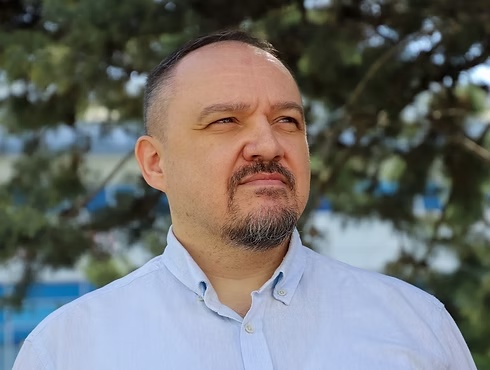
\includegraphics[width=4.5cm]{gorseller/yazar-oguz-ergin.jpg}}%
\hspace{0.7cm}%
\begin{minipage}[t]{10.5cm}%
\textbf{Prof.\ Dr.\ Oğuz Ergin}, bilgisayar mimarisi ve yüksek başarımlı işlemciler üzerine çalışan bir akademisyen, araştırmacı ve girişimcidir. Lisansını ODTÜ'de, yüksek lisans ve doktorasını New York'ta Binghamton Üniversitesi'nde tamamladı. Kariyerinin başında Intel'in Barselona araştırma merkezinde kıdemli araştırmacı olarak çalıştı; Türkiye'ye döndükten sonra TOBB ETÜ'de öğretim üyesi oldu, uzun yıllar bölüm başkanlığı ve üniversite yönetiminde danışmanlık görevleri yürüttü. 2024'ten bu yana Birleşik Arap Emirlikleri'nde Sharjah Üniversitesi Bilgisayar Mühendisliği Bölümü'nde profesör olarak görev yapmaktadır.%
\end{minipage}

\bigskip
\noindent
Araştırmaları; mikroişlemci mimarileri, bellek (özellikle DRAM) güvenliği ve güvenilirliği, enerji verimliliği, donanım hızlandırıcılar ve hata toleransı alanlarına odaklanır. Çalışmaları HPCA, MICRO ve ISCA gibi dünyadaki en saygın konferanslarda yayımlandı; 120'nin üzerinde uluslararası yayını ve çeşitli patentleri bulunmaktadır.

\medskip
\noindent
Akademi-sanayi köprüsünde aktif rol alan Ergin, Kasırga ve Yumruk şirketlerini kurarak savunma ve sivil alanlarda işlemci ve gömülü sistem çözümleri geliştirdi; Aselsan'a ve TUSAŞ'a danışmanlık yaptı ve Bilişim Vadisi'nde teknoloji danışma kurulunda görev aldı. ETH Zürih, Edinburgh ve Notre Dame üniversitelerinde misafir öğretim üyesi olarak bulundu.

\medskip
\noindent
Bugün, yetiştirdiği öğrenciler dünyanın önde gelen araştırma gruplarında ve teknoloji şirketlerinde görev alıyor; danışmanlığını yaptığı öğrenci ekipleri Teknofest yonga tasarımı yarışmalarında birçok derece elde etti. Oğuz Ergin, bilim ve teknoloji temelli yönetim anlayışını; liyakat, şeffaflık ve yüksek katma değerli üretim odaklı bir perspektifle toplumsal faydaya dönüştürmeyi amaçlıyor.


\end{document}
